\documentclass[11pt]{article}
%, a4paper

\usepackage{amsmath}\multlinegap=0pt
\usepackage{amssymb}
\usepackage[francais,english]{babel}
%\usepackage{palatino}
\usepackage{mystyle}
\usepackage{graphicx}
\usepackage{epstopdf}
\graphicspath{{./images/}}

\title{Approximation of maximal\\Cheeger sets by projection}


\author{Guillaume Carlier \\\small CEREMADE \\\small Universit\'e Paris Dauphine
                \\\small \tt carlier@ceremade.dauphine.fr \and  
     	Myriam Comte\\\small Laboratoire Jacques-Louis Lions, \\\small Universit\'{e} Pierre et Marie Curie 
				\\\small \tt comte@ann.jussieu.fr \and 
       	Gabriel Peyr\'e \\\small CEREMADE \\\small Universit\'e Paris Dauphine
                \\\small \tt peyre@ceremade.dauphine.fr
}


\begin{document}

\maketitle

\begin{abstract}
This article deals with the numerical computation of the Cheeger constant and the approximation of the maximal Cheeger set of a given subset of $\R^d$. This problem is motivated by landslide modelling as well as by the continuous maximal flow problem. Using the fact that the maximal Cheeger set can be approximated by solving a rather simple projection problem,  we propose a numerical strategy to compute maximal Cheeger sets and Cheeger constants. 
\end{abstract}

\medskip

{\textbf{Keywords}}: Cheeger sets, Cheeger constant, total variation minimization, projections. 

\clearpage


\section{Introduction}

Given $\Omega$, a Lipschitz bounded open subset of $\R^d$ and two functions $f\in L^{\infty}(\Omega)$ and $g\in C^0(\overline{\Omega})$ such that $\min(f,g)\geq c$  on $\Omega$ for some constant $c>0$, let us consider:
\begin{equation}\label{ip}
\inf\left\{\frac{\int_{\Omega} g \vert \nabla u \vert} {\int_{\Omega} f \vert u \vert  }, \; u \in W^{1,1}_0(\Omega)  \right\}.  
\end{equation}
In general, the previous problem is ill-posed, so it is natural to consider its relaxation in $BV (\Omega)$:
\begin{equation}\label{tvmin}
h(\Omega):=\inf\left\{\frac{\int_{\Omega} g d \vert D u \vert+\int_{\partial \Omega} g \vert u \vert    d \HH^{d-1}} {\int_{\Omega} f \vert u \vert  }, \; u \in BV (\Omega)  \right\}
\end{equation}
where $\HH^{d-1}$ denotes the $(d-1)$-dimensional Hausdorff measure (see \cite{eg}). The fact that the values of \pref{ip} and \pref{tvmin} are the same is well-known and follows from standard approximation results (see for instance \cite{afp}). Using the coarea formula (see \cite{eg}), it is easy to see that the quantity $h(\Omega)$ can also be expressed as
\begin{equation}\label{cheeger}
h(\Omega):=\inf\left\{ \frac{\int_{\partial^* A} g d \HH^{d-1} }{\int_A f }, \; A \subset \overline{\Omega}  \mbox{ of finite perimeter } \right\} 
\end{equation}
where $\partial^* A$ stands for the reduced boundary of $A$ (see \cite{eg}, \cite{afp}).

\smallskip

When $f\equiv g\equiv 1$, $h(\Omega)$ is known as the Cheeger constant of $\Omega$ and solutions of \pref{cheeger} are called Cheeger sets of $\Omega$, and, in this case, it can be also considered as the first eigenvalue of the degenerate $1$-Laplacian operator, see for instance Demengel \cite{dem1}, \cite{dem2}.  With weights $f$ and $g$ as above, we will again refer to $h(\Omega)$ as the  Cheeger constant and to solutions of \pref{cheeger} as Cheeger sets. In this case, the minimization problem \pref{tvmin} and the value $h(\Omega)$ are related to the  so-called maximal flow problem, see Strang \cite{strang1}, \cite{strang2} and subsection \ref{maxflow} below.

\smallskip

The existence of Cheeger sets i.e. of solutions of \pref{cheeger} is well-known and we refer the reader to \cite{cc} for the precise links between Cheeger sets and the variational problem \pref{tvmin} and various qualitative properties of solutions of \pref{tvmin}. It was recently proved in \cite{ac}-\cite{ccn}, that the Cheeger set is unique when $f\equiv g\equiv 1$ and $\Omega$ is convex.  For a general $\Omega$ and/or general weights $f$ and $g$,  Cheeger sets need not be   unique. This makes the selection of a particular Cheeger set and the numerical computation of  Cheeger constants and Cheeger sets a relevant issue, potentially important in view of applications to landslide modelling and the blocking property described in subsection \ref{landslide}. 

\smallskip

Let us consider the following closed and convex subset of $L^2(\Omega)$:
\[K=\Big\{  u\in L^2(\Omega)  \; : \;   \int_{\Omega} {\rm{ div}} (g p) u \leq 1, \; \forall p\in C^1(\Omega,\R^d), \; \Vert p \Vert_{\infty} \leq 1   \Big\}.\]
The numerical approach of the present paper is based on the fact that the projection (for some suitably weighted $L^2$ norm) of the constant function $\eps^{-1}$ onto $K$ converges as $\eps\to 0$ to a multiple of the characteristic function of the maximal Cheeger set (see \cite{bcc} and section \ref{sel} below for details). This projection problem presents of course great similarities with the famous Rudin-Osher-Fatemi problem in computer vision (\cite{rof}). Indeed, if the value of Lagrange multiplier associated to the total variation constraint was known, then one could rewrite the projection problem in the form of the Rudin-Osher-Fatemi, for which one can use for instance the algorithm of Chambolle (\cite{chambolle}). In \cite{chambolle}, Chambolle also shows how to update the Lagrange multipliers for total variation minimization with an $L^2$ equality constraint (known variance of the noise).  In our projection problem, we do not have such a consistent updating rule and it is not clear how to adapt the algorithm of Chambolle. We therefore prefer to take advantage of the special structure of the problem (projection with linear constraint) for which we can use the algorithm of Combettes and Pesquet \cite{cp}. This algorithm performs iterative sub-gradient projections in order to enforce the total variation and minimize the distance to the function $\varepsilon^{-1}$. Let us also mention the article of Alter, Caselles and Chambolle \cite{acc}, where the evolution of convex sets in the plane by the flow of the total variation is explicitly given (with some natural connections with maximal Cheeger sets) and some numerical results are obtained.


\smallskip

The paper is organized as follows. We first spend some time in section \ref{mot} to motivate the interest of problem \pref{tvmin} with general weights $f$ and $g$. More precisely, we describe two different applied settings where \pref{tvmin} and the Cheeger constant $h(\Omega)$ naturally arise: landslide modelling (\cite{cris}, \cite{hilr}, \cite{hilrr}, \cite{lri}) and the continuous maximal flow problem (see Strang \cite{strang1}, \cite{strang2}). In section \ref{sel}, we recall the results of \cite{bcc} on the selection of the maximal Cheeger set. Taking a quadratic perturbation, this gives an approximation strategy based on simple $L^2$ projection problems. The discretization of these projections is detailed, with a convergence result in section \ref{disc}. Numerical results are given in section \ref{num}. 



\section{Motivations}\label{mot}

\subsection{Landslides}\label{landslide}

In  \cite{cris}, the authors' approach to landslides modelling is to consider that  the soil  behaves like a Bingham  inhomogeneous fluid. In this model, the inhomogoneous yield limit $g$ is an important parameter in describing landslide phenomenon. Indeed, due to their own weight, the geomaterials are compacted so that their mechanical properties also vary with depth. Therefore the yield limit $g$ and the body forces $\ff$ cannot be supposed homogeneous. 

The evolution equations describing the flow of an  inhomogeneous Bingham fluid  in a domain $\D\subset\R^3$ in the time interval $(0,T)$
are 
\begin{align}
  \frac{\partial {{\boldsymbol u}} }{\partial t} + ({\boldsymbol u} \cdot \nabla) {\boldsymbol u}  -
\bfdiv \bs '
+ \nabla p &= \ff
\\
\hbox{ div } {\boldsymbol u}&=0,
\end{align}
where ${\boldsymbol u}$ is the velocity field, $\bs $ denotes
the Cauchy stress tensor field, $p =-\trace(\bs)/3$
represents the pressure and $\bs '= \bs+pI$ is the
deviatoric part of the stress tensor
and $\ff$ denotes the body forces. 
The
constitutive equation of the Bingham fluid is:
\begin{align*}
\bs' &= 2  \eta D({\boldsymbol u}) + g
\frac{D({\boldsymbol u})}{\vert  D({\boldsymbol u})\vert } \quad
& \hbox{ if } \vert  D({\boldsymbol u})\vert \neq 0,
\\ 
\vert \bs' \vert &\le g & \hbox{ if } \vert
D({\boldsymbol u})\vert = 0,
\end{align*}
%
where $D({\boldsymbol u}) = (\nnabla {\boldsymbol u} + \nnabla^T
{\boldsymbol u})/2$, $\eta(x) \ge \eta_0>0$ 
is the viscosity distribution and $g=g(x) >
0 $ on $\clos \D$ is the (non homogeneous)
yield limit distribution in $\D$. 

The boundary conditions are  
${\boldsymbol u} = 0$  on $\partial\D\times
(0,T)$ and  ${\boldsymbol u} \vert_{t=0}= {\boldsymbol u}_0$. Writing the problem under variational form leads to 
\begin{equation} \label{time-ineq}
\begin{aligned}
&\int_\D  \Bigl(
\frac{\partial {{\boldsymbol u}} }{\partial t} + ({\boldsymbol u} \cdot
\nabla) {\boldsymbol u} \Bigr) \cdot (\bv - {\boldsymbol u})
+ \int_\D 2 \eta D({\boldsymbol u}) . (D(\bv)- D({\boldsymbol u}))
\\
&+ \int_\D g (\vert D(\bv)\vert   - 
\vert D({\boldsymbol u})\vert)  
\ge \int_\D  \ff \cdot
(\bv - {\boldsymbol u}) .
\end{aligned}
%\right.
\end{equation}
for all $t\in(0,T)$,  ${\boldsymbol u}$ and $\bv $ in some suitable space, see \cite{duli} . If we consider the stationary 
\emph{anti-plane} flow, that is  $\D=\Omega\times\R$ with $\Omega$ open domain of $\R^2$ with lipschitz boundary,  
${\boldsymbol u}=(0,0,u(x_1,x_2))$ and similar hypotheses for $\ff$,
etc. Problem (\ref{time-ineq}) then becomes
\begin{eqnarray}
%\begin{split}
%u \in V, \qquad \forall v \in V,\\
\intO 
2\eta(x)\nabla u(x)
\cdot \nabla (v(x)-u(x)) \, dx\nonumber 
+ \intO g(x) (\vert \nabla v(x)\vert - \vert
\nabla u(x)\vert \,) dx\\
\ge \intO
f(x)(v(x)-u(x)) \, dx \label{vfap}.
%\end{split}
\end{eqnarray}
for all $u,v$ in some suitable functional space, see \cite{hilrr}. 
Since $u$ is the velocity of the fluid, the Bingham fluid is blocked, that is there is no landslide, if $u\equiv0$ is a solution of (\ref{vfap}). Hence the blocking property reads as 
%\begin{equation}\label{ineq-base}
%\intO g(x) \vert \nabla v(x) \vert \, dx \ge \intO f(x)v(x) \,
%dx, \quad  \forall v \in V.
%\end{equation}
%ou de fa\c con \'equivalente
\begin{equation}\label{BSV}
1\leq \mu:= \inf_{v \in  W^{1,1}_0(\Omega)} 
 \frac{\displaystyle \intO g(x) \abs{
\nabla v (x)} \, dx}{ \left\vert \displaystyle\intO f(x) v(x)
\,dx  \; \right\vert}.
\end{equation}%
Thus $\mu$ has been considered in \cite{hilr} as a safety factor and it is important to know for given $f$ and $g$, if $\mu$ is larger than $1$ (blocking property).


\subsection{Maximal flow, minimum cut duality and Cheeger sets}\label{maxflow} 

Another motivation for \pref{tvmin} comes from its relation with the so-called maximal flow problem. The duality between \pref{ip} and the continuous maximal flow problem is essentially due to Strang \cite{strang1}. We refer to the papers of Strang \cite{strang1} and \cite{strang2}  for a detailed exposition of the problem, extensions and related questions. This continuous duality is used by Appleton and Talbot \cite{appleton} to solve computer vision problems such as image segmentation.

First, it is easy to see that 
\begin{equation}
-\frac{1}{h(\Omega)}= \inf\{F(u)+H(\nabla u)\; : \; u\in W^{1,1}_0(\Omega)\}
\end{equation}
where 
\[F(u)=-\int_{\Omega} fu, \; H(\bq)=\left\{\begin{array}{ll}
  0  &\hbox{ if } \Vert g  \bq \Vert_{L^1}=\int_{\Omega} g \vert \bq \vert \leq 1\\
+\infty &\hbox{ otherwise},
\end{array}\right.\]
forall  $u\in  W^{1,1}_0(\Omega)$ and $\bq \in L^{1}(\Omega, \R^d)$. Since $F$ and $G$ are convex l.s.c. functionals with $F$ everywhere finite and $G$ continuous at $0$, the Fenchel-Rockafellar duality theorem (see Ekeland and Temam \cite{ektem}) yields
\[\frac{1}{h(\Omega)}=\min \{ F^*(-\div(\bv))+H^*(-\bv), \; \bv\in L^{\infty}(\Omega,\R^d)\}\]
where $F^*$ and $H^*$ denote the Fenchel conjugates of $F$ and $H$. By direct computation, we then get:
\[\frac{1}{h(\Omega)}=\min\left\{ \left\Vert  \frac{\bv}{g} \right\Vert_{L^{\infty}}\; : \; \bv\in L^{\infty}(\Omega,\R^d), \; \div(\bv)=f  \right\}.\]
Which enables us to rewrite the Cheeger constant as
\begin{equation}\label{duality}
h(\Omega)=\max\left\{ \lambda\in \R \; :  (\lambda, \bv)\in \R\times L^{\infty}(\Omega,\R^d),   \; \div(\bv)=\lambda f, \; \vert \bv \vert \leq g \right\}.
\end{equation}
The duality relation \eqref{duality} is known as the maximal flow-minimal cut theorem. The maximization problem in \pref{duality} is a continuous version of the problem that consists in finding the largest flow that can be sent  through the edges of a graph given their capacity (the function $g$ in a continuous setting) and subject to the mass conservation constraint (Kirchoff's law on a graph and $\div(\bv)=\lambda f$ in a continuous setting).  The natural assumption on $f$ is that it has zero average and can be written as $f=f^+-f^{-}$  with $f^+$ and $f^-$ giving the distribution of sinks and sources. Also, the maximal flow problem described above is isotropic in the sense that the capacity constraint simply is $\vert \bv \vert \leq g$ and does not depend on the direction of the flow, we refer to Nozawa \cite{nozawa} for a general anisotropic formulation.   As usual in convex duality, one expects useful relations between maximal flows and all the solutions of the primal problem (in particular characteristic functions of Cheeger sets).  In fact, it follows from the maximal flow-minimal cut theorem that if $C$ is a Cheeger set and $\bv$ a maximal flow  then  (at least formally, i.e. ignoring regularity issues) $\bv \cdot n =g$ on $\partial C$. Therefore $\partial C$ is filled to its maximum capacity, $\partial C$ is then refered to as a \emph{minimum cut}. 


\section{Selection of the maximal Cheeger set}\label{sel}

As already pointed out, Cheeger sets i.e. solutions of \pref{cheeger} are non-unique in general, however  there exists a unique maximal Cheeger set i.e. a solution of \pref{cheeger} that contains any other one up to a negligible set. We refer to \cite{bcc} for a proof of the next result:


\begin{prop}
There exists a unique maximal Cheeger set, i.e. a unique $C_0$ solving \pref{cheeger} such that for every $C$ solving \pref{cheeger}, $C$ is included in $C_0$ up to a Lebesgue negligible set.
\end{prop}
 
In \cite{bcc},  the question of whether some natural perturbations of \pref{tvmin} select at the limit the maximal Cheeger set is addressed. In particular, if we rewrite the Cheeger constant as
\begin{equation}\label{cheeger1}
\frac{1}{h(\Omega)}= \sup\Big\{\int_\Omega f  u \, dx \ :\ \int_{\Omega} g\,d|Du| +\int_{\partial \Omega} g \vert u \vert    d \HH^{d-1}  \le1,\ u\in BV(\Omega)\Big\}
\end{equation}
Following the approach of  \cite{bcc}, we approximate \pref{cheeger1} by the strictly concave penalization
\begin{equation}\label{cheegereps}
\sup\Big\{\int_\Omega f\big(u-\eps\Phi(u)\big)\,dx\ :\ 
\int_{\Omega} g\,d|Du| +\int_{\partial \Omega} g \vert u \vert    d \HH^{d-1}  \le1,\ u\in BV(\Omega)      \Big\}
\end{equation}
where $\eps>0$ is a perturbation parameter and $\Phi$ is a strictly convex even function that satisfies
\begin{equation}\label{grc}
\Phi(0)=0,\qquad 0\le\Phi(t)<+\infty\quad\forall t\in\R^+.
\end{equation}
Denoting by $\chi_A$ the characteristic function of a set $A$, the following convergence\footnote{the fact that we do not have to impose any growth condition on $\Phi$ comes from the fact that solutions of \pref{tvmin} are all $L^{\infty}$, see \cite{cc}.} result states that solutions of the penalized problems converge to a multiple of the characteristic function of the maximal Cheeger set (see \cite{bcc} for a proof).

\begin{thm}\label{cvgcc}
Let $u_\eps$ be the unique solution of \eqref{cheegereps}. Then $(u_\eps)_\eps$ converges in $L^1(\Omega)$, as $\eps\to0^+$, to $\ovu=\alpha\chi_{C_0}$,  where $\alpha>0$ and $C_0\subset\Omb$ is the maximal Cheeger set.
\end{thm}

A natural choice for the perturbation $\Phi$ is of course 
\[\Phi(t):= \frac{t^2}{2} \]
in which case, the perturbed problem \pref{cheegereps} is easily seen to be equivalent to the projection problem
\begin{equation}\label{proj}
\inf \Big\{\int_\Omega f\Big(u-\frac{1}{\eps}\Big)^2 \,dx\ :\ 
\int_{\Omega} g\,d|Du| +\int_{\partial \Omega} g \vert u \vert    d \HH^{d-1}  \le1,\ u\in BV(\Omega)      \Big\}
.\end{equation}
The solution of the previous problem $u_{\eps}$ can of course be expressed as
\begin{equation}\label{proj2}
u_{\eps}= \Pi_K\Big(\frac{1}{\eps}\Big)
\end{equation}
where $\Pi_K$ denotes the projection (for the weighted $L^2$ inner product $(u,v):=\int_{\Omega} f u v$) on the closed subset $K$ of $L^2(\Omega)$ defined by
\begin{equation}\label{defK}
K:=\Big\{  u\in L^2(\Omega)\cap BV(\Omega)  \; : \;    \int_{\Omega} g\,d|Du| +\int_{\partial \Omega} g \vert u \vert    d \HH^{d-1}  \le1 \Big\}.
\end{equation}
It is convenient to extend every $u\in BV(\Omega)$  (or $L^2(\Omega)$) by $0$ outside $\overline{\Omega}$, doing so we have: 
\[ \int_{\Omega} g\,d|Du| +\int_{\partial \Omega} g \vert u \vert    d \HH^{d-1} =\int_{\R^d}  g\,d|Du|.\]
If we further assume that $g\in C^1(\overline{\Omega})$ then it is well-known that $K$ can be described by a set of linear  constraints as follows
\begin{equation}\label{carK}
K=\Big\{  u\in L^2(\Omega)  \; : \;   \int_{\Omega} {\rm{ div}} (g p) u \leq 1, \; \forall p\in C^1(\Omega,\R^d), \; \Vert p \Vert_{\infty} \leq 1   \Big\}.
\end{equation}


\section{Discretization and projection}\label{disc}

\subsection{Discretization}


We aim now to discretize our projection problem to approximate the projection $u_{\eps}=\Pi_K\Big(\frac{1}{\eps}\Big)$ with $K$ defined by \pref{carK}. For the sake of simplicity, we shall from now on assume that the ambient space dimension is $d=2$ and that $\Omega=(0,1)^2$. 
More generally, given $u^0\in L^2(\Omega)$, we are interested in projecting $u^0$ onto $K$ i.e.
\begin{equation}\label{proju}
\inf_{u\in K} F(u)=\int_{\Omega} f(u-u^0)^2\
\end{equation}
with $K$ defined as before by $K=\{u\in BV(\Omega)\;  : \; G(u)\leq 1\}$ where
\[G(u):=\int_{\Omega} g\,d|Du| +\int_{\partial \Omega} g \vert u \vert    d \HH^{d-1}.\] 
We assume that the weights $f$ and $g$ are respectively continuous and $C^1$ on some neighbourhood of $\Omega$ and bounded by below by some strictly positive constant.
We denote by $\Pi_K(u^0)$ the solution of \pref{proju}.
Given a step size $h=1/N$, we then consider the following discretization of \pref{proju}. First, let $E_h$ be the set of matrices $u$ with entries $u_{i,j}$, $i,j\in\{0,N\}^2$, by convention we extend $u$ by setting $u_{i,j}=0$ when either $i$ or $j$ belongs to $\{-1,N+1\}$. For $u=(u_{i,j})_{ij}\in E_h$ we set
\[\partial_x^h u_{i,j}:=\left\{\begin{array}{ll}
h^{-1}(u_{i+1,j}-u_{i,j})  & \mbox{ if }   -1\leq i\leq N,\; -1\leq  j\leq N-1\\
0  & \mbox{ if }   -1\leq i\leq N,\;  j=N.
\end{array}\right.\]
\[\partial_y^h u_{i,j}:=\left\{\begin{array}{ll}
h^{-1}(u_{i,j+1}-u_{i,j})   & \mbox{ if }   -1\leq i\leq N-1 ,\; -1\leq  j\leq N \\
0, \;   & \mbox{ if }   -1\leq j\leq N,\;  i=N.
\end{array}\right.\]
We also set $\nabla^h u_{i,j}=(\partial_x^h u_{i,j},\partial_y^h u_{i,j})$. Denoting $f_{ij}^h$ and $g_{ij}^h$ some discrete approximation of the weights $f$ and $g$ (e.g. $f_{i,j}^h=f(ih,jh)$, $g_{i,j}^h=g(ih,jh)$)  and $u^0_{i,j}$ some discretization of $u^0$ (approximation by mean values say) we then discretize $G$ by definining, for all $u\in E_h$:
\[G_h(u):= h^2\sum_{i=-1}^N \sum_{j=-1}^N  g_{i,j}^h \vert \nabla^h u_{i,j}\vert\]
which can be rewritten as
\[\begin{split}
&G_h(u) = h^2\sum_{i=0}^{N-1} \sum_{j=0}^{N-1}  g_{i,j}^h \vert \nabla^h u_{i,j}\vert\ \\
&+ h\sum_{i=0}^{N}\left( g_{i,-1}^h  \vert u_{i,0}\vert+g_{i,N}^h\vert u_{i,N}\vert \right) +h\sum_{j=0}^{N}\left( g_{-1,j}^h \vert u_{0,j}\vert+ g_{N,j}^h \vert u_{N,j}\vert  \right).\end{split}\]
Defining $K_h$ by $K_h:=\{u\in E_h \; : \; G_h(u)\leq 1\}$ and 
\[F_h(u):= h^2 \sum_{i=0}^{N-1} \sum_{j=0}^{N-1} f_{i,j}^h (u_{i,j}-u^0_{i,j})^2,\]
we then approximate \pref{proju} by 
\begin{equation}\label{projuh}
\inf_{u\in K_h} F_h(u) 
\end{equation}
and denote by $u^h$  the solution of \pref{projuh}.  Denoting  by $C_{ij}$ the square $(ih,(i+1)h)\times(jh,(j+1)h)$, we define  $v_h$ as the piecewise constant function  having value $u^h_{i,j}$ on $C_{ij}$.  Denoting by $\M(\overline{\Omega},\R^2)$ the space of bounded $\R^2$-valued measures on $\overline{\Omega}$, we then have the following convergence result.

\begin{thm}
Let $v_h$ be defined as above, then $v_h$ converges to $\Pi_K(u_0)$ strongly in $L^2(\Omega)$ and $\nabla v_h$ converges weakly $\star$ to  $\nabla \Pi_K(u_0)$ in $\M(\overline{\Omega},\R^2)$ as $h\to 0$. 
\end{thm}

\begin{proof}
It is easy to see that $(v_h)_h$ is bounded in $BV$ and in $L^2$ hence admits a (not relabeled) subsequence that strongly converges in $L^1$ and weakly in $L^2$ to some $v\in BV\cap L^2$ and such that  $\nabla v_h$ converges to $\nabla v$ weakly $\star$  in $\M(\overline{\Omega},\R^2)$. Let us prove that $v\in K$, i.e. (recalling \pref{carK})
\[\int_{\Omega} {\rm{div}}(gp) v\leq 1\]
for every $p\in C^1(\overline{\Omega},\R^2)$ such that $\Vert p \Vert_{\infty}\leq 1$. For such a $p=(p^1,p^2)$ we obviously have
\[\int_{\Omega} {\rm{div}}(gp) v=\lim_h h \left( \sum_{j=0}^{N-1} \sum_{i=0}^N (a_{i,j}-a_{i-1,j})u_{i,j}^h 
+   \sum_{i=0}^{N-1} \sum_{j=0}^N (b_{i,j}-b_{i,j-1})u_{i,j}^h    \right) \]
where we have set 
\[a_{i,j}=g_{ij} p^1(ih,jh) \mbox{ and } b_{i,j}=g_{ij} p^2(ih,jh).\]
Rearranging terms, we  have
\[\begin{split}
&h \left( \sum_{j=0}^{N-1} \sum_{i=0}^N (a_{i,j}-a_{i,j-1})u_{i,j}^h
+   \sum_{i=0}^{N-1} \sum_{j=0}^N (b_{i,j}-b_{i,j-1})u_{i,j}^h    \right)\\
&=-h^2  \sum_{i=0}^{N-1} \sum_{i=0}^{N-1}  (a_{i,j},b_{i,j})\cdot \nabla^h u_{i,j}^h 
+h \sum_{i=0}^{N-1} (b_{i,N}u_{i,N}^h-b_{i,-1} u_{i,0}^h)\\
&+h \sum_{j=0}^{N-1} (a_{N,j}u_{N,j}^h-a_{-1,j} u_{0,j}^h)\end{split}\]
we thus deduce from $\vert (a_{i,j},b_{i,j})\vert\leq g_{i,j}$ and the continuity of $g$
\[\int_{\Omega} {\rm{div}}(gp) v \leq \limsup_h G_h(u^h)\leq 1\]
which proves that $v\in K$.

\smallskip

Let us now prove that $v=\Pi_K(u^0)$. Let $\varphi\in C^1(\Omb)\cap K$ and $\varphi_h$ be the affine interpolate of $\varphi$ on the triangles $(T_{ij}^+, T_{ij}^-)$ where $T_{ij}^-$ has vertices $(ih,jh)$, $((i+1)h,jh)$ and $(ih, (j+1)h)$ and $T_{ij}^+$ is the complement of $T_{ij}^-$ in $C_{ij}$. It is obvious that
\[G(\varphi)=\lim_h G_h(\varphi_h)\]
hence for every $\delta>0$, $\varphi_h/(1+\delta)\in K_h$ for $h$ small enough. We then have (also denoting by $\varphi_h$ the values of $\varphi$ at the nodes)
\[F_h(v_h)\leq F_h\left(\frac{\varphi_h}{1+\delta}\right)\]
and then 
\[F(v)\leq \liminf_h F_h(v_h)\leq  \liminf_h  F_h\left(\frac{\varphi_h}{1+\delta}\right)=F\left(\frac{\varphi}{1+\delta}\right).\]
Since $\delta>0$ is arbitrary we deduce that $F(v)\leq F(\varphi)$ for every $\varphi\in C^1(\Omb)\cap K$, it then follows from standard approximation arguments in  $BV$ (see in particular remark 3.22 p.132 in \cite{afp}) that $v=\Pi_K(u^0)$. It is then easy to check that $\Vert v_h\Vert_{L^2}$ converges to $\Vert v \Vert_{L^2}$, so that by classical arguments the whole sequence $v_h$ converges strongly in $L^2$ to $v=\Pi_K(u^0)$. 

\end{proof}

%%%%%%%%%%%%%%%%%%%%%%%%%%%%%%%%%%%%%%%%%%%%%%%%%%%%%%%%%%%%%%%%%%
%%%%%%%%%%%%%%%%%%%%%%%%%%%%%%%%%%%%%%%%%%%%%%%%%%%%%%%%%%%%%%%%%%
%%%%%%%%%%%%%%%%%%%%%%%%%%%%%%%%%%%%%%%%%%%%%%%%%%%%%%%%%%%%%%%%%%
\subsection{Algorithm for the discrete projection problem}
\label{subsec-algorithm}

The projection \eqref{projuh} of the discretized problem is computed numerically using the iterative algorithm of Combettes and Pesquet \cite{cp}. It corresponds to a subgradient projection method that only requires, at each iteration, the projection of the current estimate on the intersection of two half spaces. The iterative algorithm \cite{cp} needs to be modified to take into account the weight $f$ in the least square objective function. We thus use the algorithm to compute the projection of $\sqrt{f}u_0$ where $u_0=\varepsilon^{-1}$.

We now detail the steps of this algorithm. For clarity we drop the dependancies on the grid size $h=1/N$ of the processed vectors.
\begin{enumerate}
	\item \textit{Initialization.} Set $u^{(0)} = \sqrt{f} u_0$ and set $k \leftarrow 0$.
	\item \textit{Sub-gradient computation:} Define the sub-gradient of the total variation at the current iterate as
		\begin{align}\label{eq-subgradient-tv}
			t^{(k)} & = \frac{1}{\sqrt{f}}\div( g p^{(k)} )\\
			\text{with}\quad
			p^{(k)}_{i,j} & = 
			\left\{
			\begin{array}{l}			
			\frac{ \nabla \tilde u^{(k)}_{i,j} }{ \norm{\nabla \tilde u^{(k)}_{i,j}}} \;\text{ if }\; 
				\nabla \tilde u^{(k)}_{i,j} \neq 0,\\
			0 \quad \text{otherwise}.
			\end{array}
			\right.
		\end{align}
		where $\tilde u = u / \sqrt{f}$.
	\item \textit{Sub-gradient projection computation.} Define
		\begin{equation*}
			z^{(k)} = 
			\left\{
			\begin{array}{l}
				u^{(k)} - ( G(\tilde u^{(k)}) - 1  ) \frac{t^{(k)}}{\norm{t^{(k)}}^2} 
				\quad\text{if}\quad G(\tilde u^{(k)}) > 1, \\
				u^{(k)} \quad \text{otherwise}.
			\end{array}
			\right.
		\end{equation*}
		as the sub-gradient projection of the current estimate.
	\item \textit{Projection onto half-spaces.} Define the two half spaces
		\begin{align*}
			D^{(k)} &= \enscond{ v }{ \dotp{u^{(k)}-v}{u^{(k)}-u^{(0)}} \leq 0 }, \\
			H^{(k)} &= \enscond{ v }{ \dotp{v-z^{(k)}}{u^{(k)}-z^{(k)}} \leq 0 }.
		\end{align*}
		The new iterate is defined as the following projection 
		\begin{equation}\label{eq-update-estimate}
			u^{(k+1)} = \Pi_{ D^{(k)} \cap H^{(k)} } \left( u^{(0)} \right).
		\end{equation}
	\item \textit{Boundary correction.} Constrain the current estimate to vanish outside $\Omega$ by defining
		\begin{equation*}
			u^{(k+1)}_{i,j} = 
			\left\{
			\begin{array}{l}
				u^{(k+1)}_{i,j} \quad\text{if}\quad (i,j)/N \in \Omega,\\
				0 \text{ otherwise. }
			\end{array}
			\right.
		\end{equation*}
	\item \textit{Stopping criterion.} While $\norm{u^{(k-1)}-u^{(k)}} > Tol$, set $k \leftarrow k+1$ and go back to 2.
	If the algorithm has converged, return $u = u^{(k)}/\sqrt{f}$.
\end{enumerate}

As shown in \cite{cp}-\cite{comb}, the iterates $u^{(k)}/\sqrt{f}$ converge when $k \rightarrow +\infty$ to the solution $u^h$ of the discrete optimization problem \eqref{projuh}. The algorithm is stopped when $\norm{u^{(k-1)}-u^{(k)}}$ is smaller than a given tolerance value $Tol$. 

Let us remark that, by construction, $D^{(k})\cap H^{(k)}$ contains $\sqrt{f}K=\{v \; : \; G(\tilde{v}) \leq 1\}$ hence is nonempty. Indeed (taking $f=1$ for the sake of simplicity and without loss of generality) let $v\in K$ and let us prove that $v\in H^{(k)}$. If $G(u^{(k)})\leq 1$, there is nothing to prove, we may then assume that $G(u^{(k)})>1$,  since $t^{(k)}\in \partial G (u^{(k)}))$, we have
\[ \dotp{v-z^{(k)}}{ t^{(k)}}= \dotp{v-u^{(k)}}{ t^{(k)}}+ \dotp{u^{(k)}-z^{(k)}}{t^{(k)}} \leq G(v)-1\leq 0\]
so that $v\in H^{(k)}$. Now assume that $v\in D^{(k)}$ (which is the case for $k=0$), since $u^{(k+1)}$ is the projection of $u^{(0)}$ on $D^{(k)}\cap H^{(k)}$, we have
\[\dotp{u^{(k+1)}-v} {u^{(k+1)}-u^{(0)}}\leq 0\]
hence $v\in D^{(k+1)}$.

\smallskip

The main step of the algorithm is the computation of \eqref{eq-update-estimate} which is an euclidean projection on the (nonempty) intersection of two half spaces. As explained in \cite{comb}, such a projection is computed as follows.

\begin{lem} Let $u,u_0$ and $z$ be vectors in $\mathbb{R}^n$ and define the half planes
\begin{equation*}
			D = \enscond{ v }{ \dotp{u-v}{u-u_0} \leq 0 }
			\quad\text{and}\quad
			H = \enscond{ v }{ \dotp{v-z}{u-z} \leq 0 }.
\end{equation*}
Let $\pi = \dotp{u_0-u}{u-z}$, $\mu = \norm{u_0-u}^2$, $\nu = \norm{u-z}^2$ and $\rho = \mu\nu-\pi^2$. If $D\cap H\neq \emptyset$, the orthogonal projection of $u_0$ on $D \cap H$ satisfies
\begin{equation*}
	\Pi_{D \cap H}(u_0) = 
			\left\{
			\begin{array}{l}
				z \text{ if } \rho=0 \text{ and } \pi\geq 0, \\
				u_0 + (1+\pi/\nu)(z-u) \text{ if } \rho > 0 \text{ and } \pi\nu \geq \rho, \\
				u + \frac{\nu}{\rho}\left( \pi(u_0-u) + \mu(z-u) \right)  \text{ if } \rho > 0 \text{ and } \pi\nu \leq \rho.
			\end{array}
			\right.
\end{equation*}
\end{lem}

\newcommand{\myrot}[1]{\rotatebox{90}{\qquad\;#1}} % \hspace{-2mm}

\myfigure{
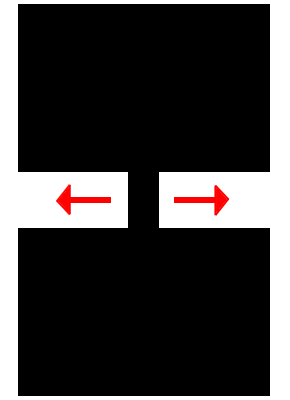
\includegraphics[width=.215\linewidth]{cheeger-2d/square-tube-original.png}\hspace{-2mm}
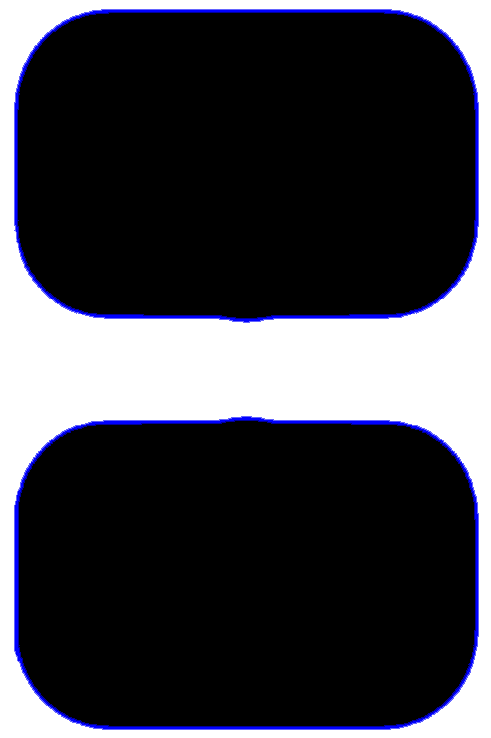
\includegraphics[width=.2\linewidth]{cheeger-2d/square-tube-26-l2-cheeger-curve.png}\hspace{-2mm}
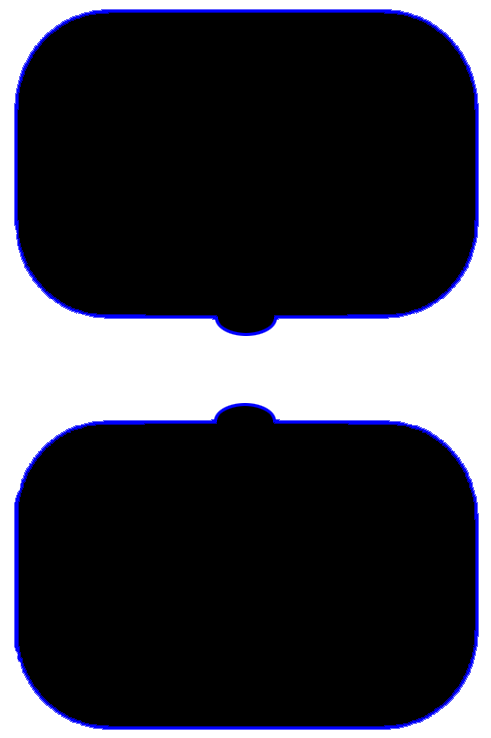
\includegraphics[width=.2\linewidth]{cheeger-2d/square-tube-31-l2-cheeger-curve.png}\hspace{-2mm}
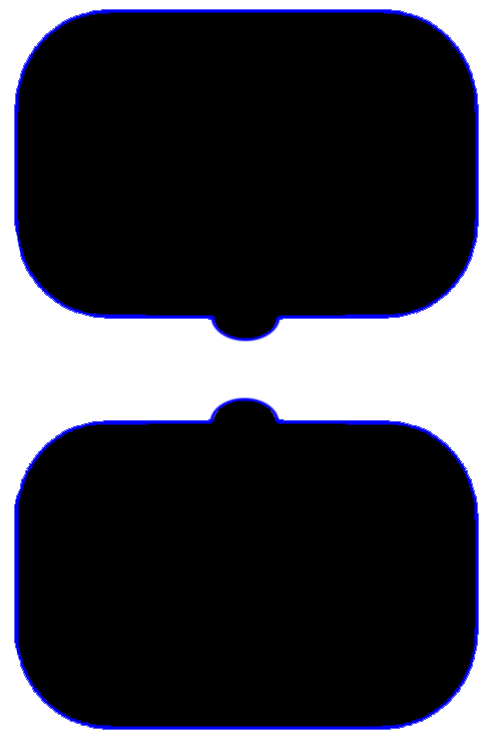
\includegraphics[width=.2\linewidth]{cheeger-2d/square-tube-35-l2-cheeger-curve.png}\hspace{-2mm}
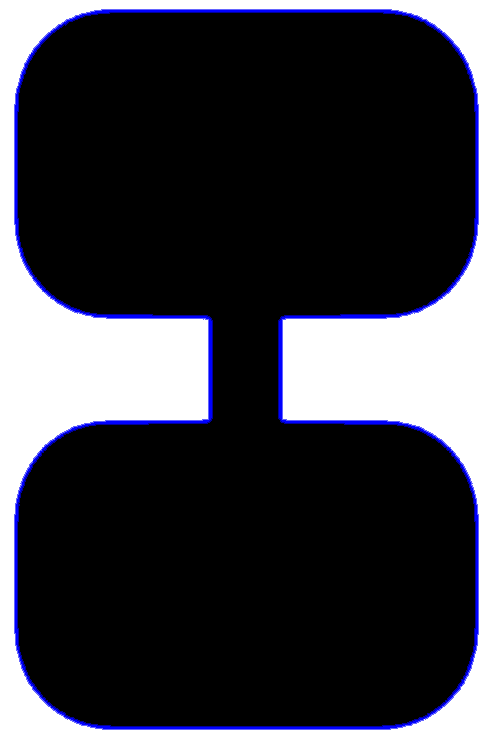
\includegraphics[width=.2\linewidth]{cheeger-2d/square-tube-39-l2-cheeger-curve.png}
}{
The original shape is composed of two rectangles linked with a tube of increasing width. The corresponding Cheeger sets are displayed on the right.
}{fig-cheeger-square-tube}


%%%%%%%%%%%%%%%%%%%%%%%%%%%%%%%%%%%%%%%%%%%%%%%%%%%%%%%%%%%%%%%%%%
%%%%%%%%%%%%%%%%%%%%%%%%%%%%%%%%%%%%%%%%%%%%%%%%%%%%%%%%%%%%%%%%%%
%%%%%%%%%%%%%%%%%%%%%%%%%%%%%%%%%%%%%%%%%%%%%%%%%%%%%%%%%%%%%%%%%%
\section{Numerical results}\label{num}

For the numerical experiments, we have used $\varepsilon = 1/100$ which results in an approximate solution $u_\varepsilon$ with sharp transitions. The discretization step size $h=1/N$ is set with $N=400$ for $d=2$ (2D computations) and $N=50$ for $d=3$ (3D computations). 

\paragraph{Convergence study.}

The convergence of our projection algorithm is studied for a square domain $\Omega$ of unit side length, for $f=g=1$. In this case, the Cheeger set $C_0$ is unique and known, since it is composed of parts of the square edges and arcs of a circle of radius $(2+\sqrt{\pi})^{-1}$, as shown in Figure \ref{fig-cheeger-bump}, left. Figure \ref{fig-cheeger-bump}, right, shows the convergence of the iterates $u^{(k)}$ toward the normalized indicator function $\alpha \chi_{C_0}$, where $\alpha = \frac{1}{|\partial^* C_0|}$. The $L^\infty$ error converges toward a non-zero residual error $\norm{ \alpha \chi_{C_0} - u^{(+\infty)} }_{\infty}$ that decreases if the value $\varepsilon$ is reduced.

\myfigure{
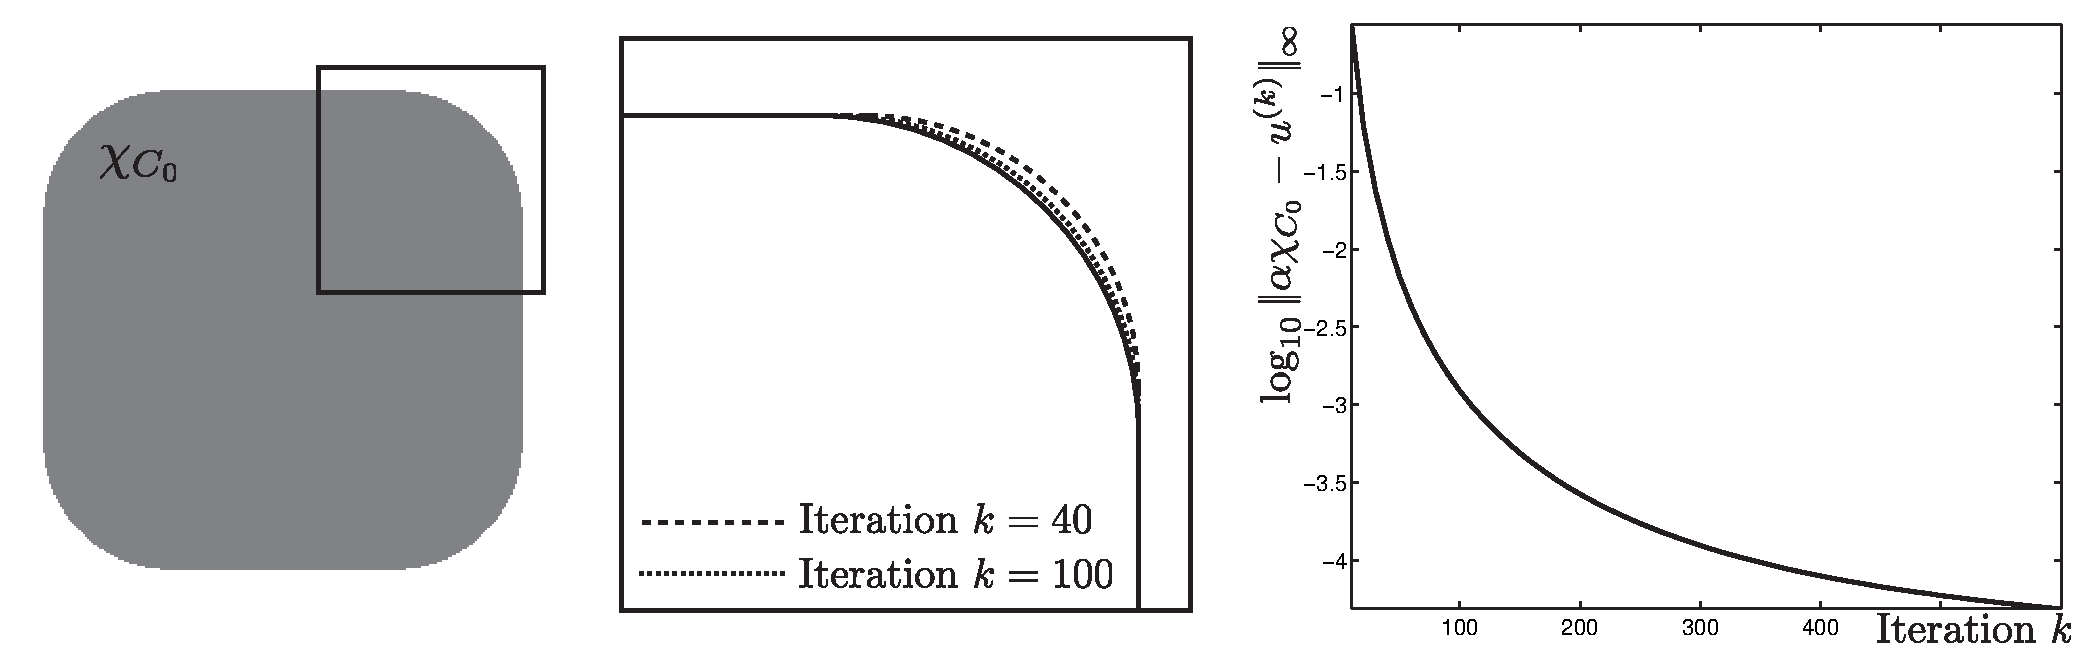
\includegraphics[width=\linewidth]{error/square-cheeger-progression.eps}
}{
Left: Cheeger set $C_0$ of a square. Center: zoom on the exact Cheeger boundary $\partial^* C_0$ together with the curves extracted by our algorithm after $k=40$ and $k=100$ iterations (dotted line). Right: convergence of the $L^\infty$ error $\log_{10} \norm{ \alpha \chi_{C_0} - u^{(k)} }_{\infty}$ during the iterations of the projection algorithm.
}{fig-cheeger-bump}

\paragraph{Cheeger sets in 2D and 3D.}

Figure \ref{fig-cheeger-square-tube} shows the extraction of the Cheeger set for two squares connected by a rectangle of increasing width. Our algorithm is able to extract the maximum Cheeger although these shapes do not have an unique Cheeger. Figure \ref{fig-cheeger-2d} (second column) shows examples of Cheeger sets for 2D shapes and for constant weights $f=g=1$. In these examples, the original domain $\Omega$ is non-convex, and the projection algorithm correctly identifies the maximum Cheeger set.

Our projection algorithm works in arbitrary dimension $d$, and Figure \ref{fig-cheeger-3d} shows examples of Cheeger sets for 3D shapes with constant weights $f=g=1$.


\paragraph{Cheeger sets with non-constant weights.}

Figure \ref{fig-cheeger-bump} shows examples of Cheeger sets for a non-constant weight $g$. This particular choice of weight (a gaussian bump with a varying position) causes the boundary of the Cheeger set to deviate from its original position for $g=1$. Figure \ref{fig-cheeger-weight} shows others examples of non-constant weights $f$ and $g$. 



\myfigure{
\myrot{Shape}
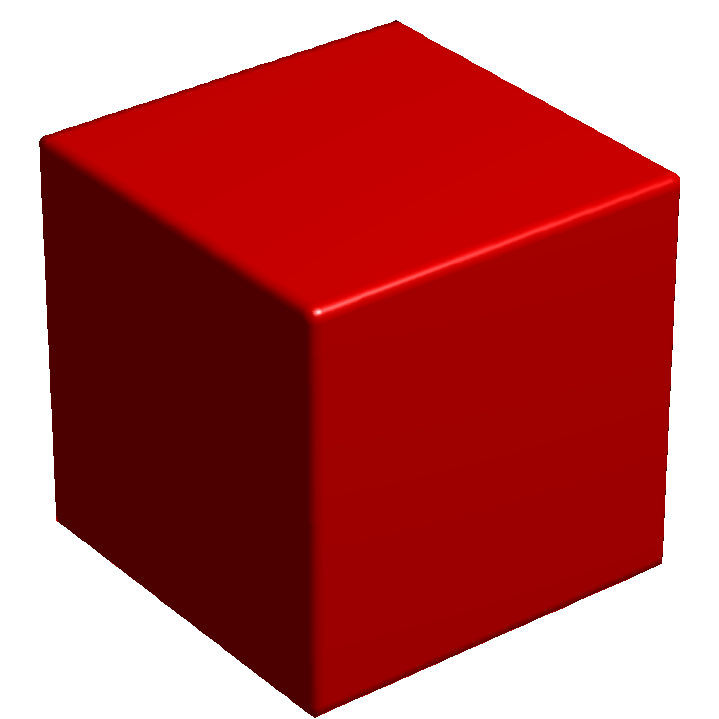
\includegraphics[width=.31\linewidth]{cheeger-3d/cube-shape.png}
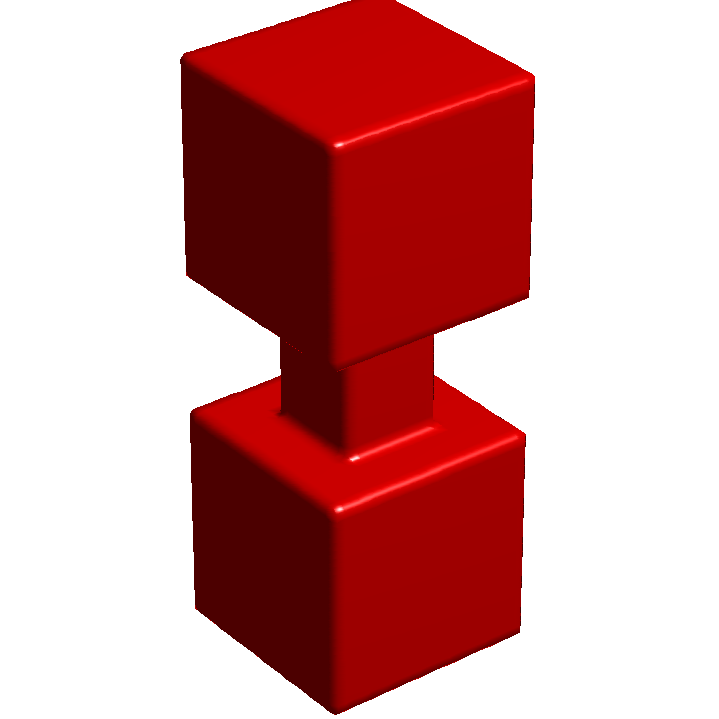
\includegraphics[width=.31\linewidth]{cheeger-3d/cubes-tube-shape.png}
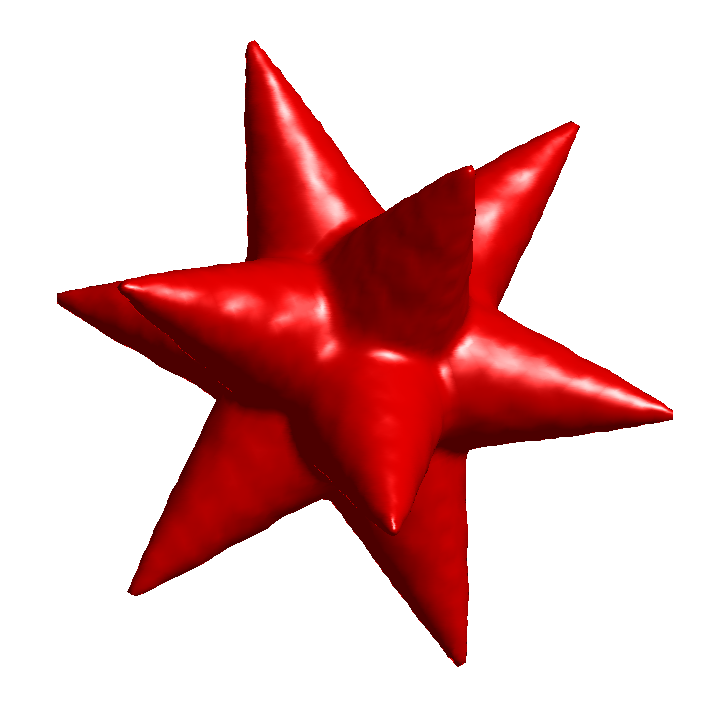
\includegraphics[width=.31\linewidth]{cheeger-3d/multi-cones-shape.png}\\
\myrot{Cheeger}
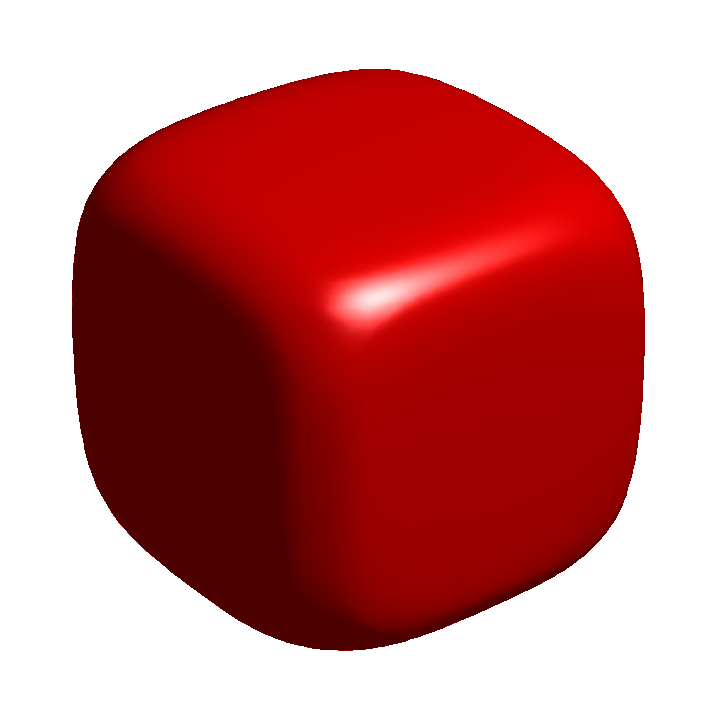
\includegraphics[width=.31\linewidth]{cheeger-3d/cube-cheeger.png}
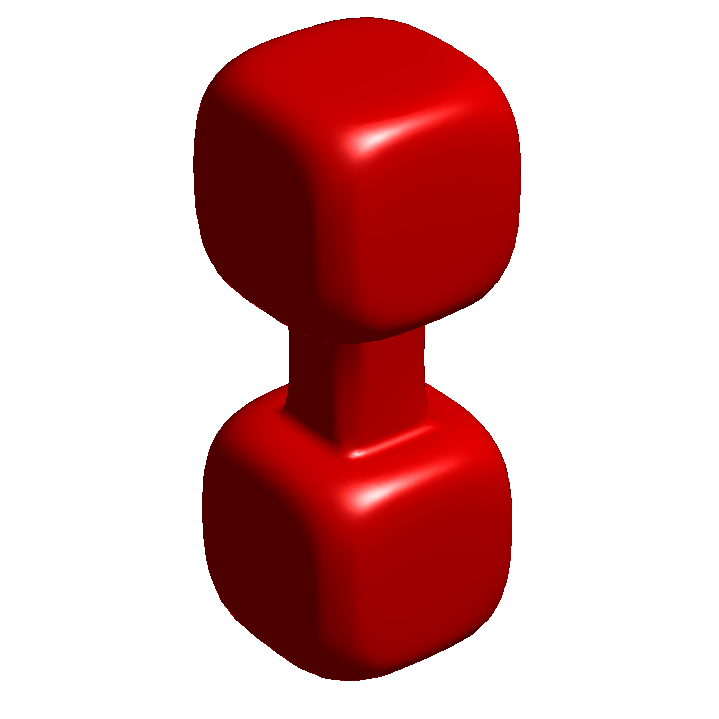
\includegraphics[width=.31\linewidth]{cheeger-3d/cubes-tube-cheeger.png}
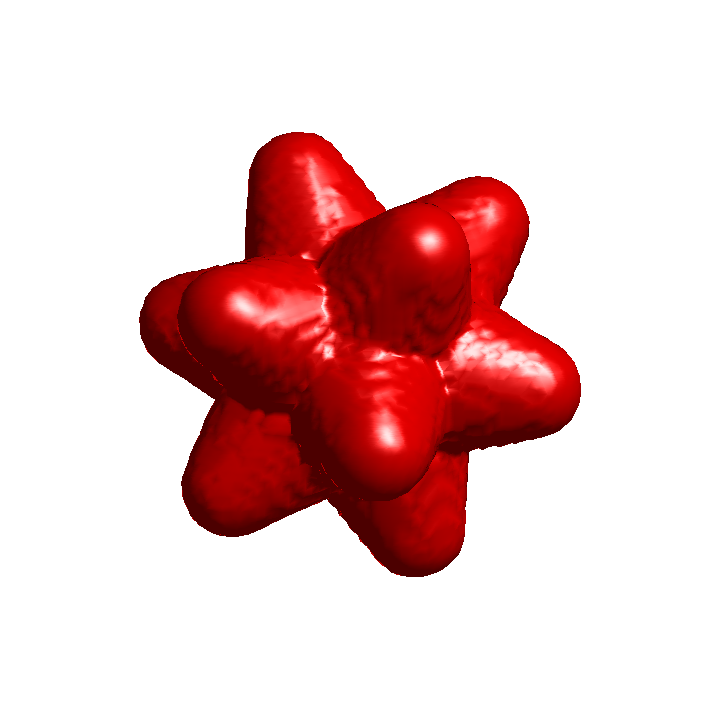
\includegraphics[width=.31\linewidth]{cheeger-3d/multi-cones-l2-cheeger.png}\vspace{-3mm}
}{
Cheeger sets in 3D with constant weights $f=g=1$.
}{fig-cheeger-3d}

\myfigure{
\myrot{Weight $g$}

\includegraphics[width=.22\linewidth]{cheeger-weight/square-constant-bump4-tv.png}

\includegraphics[width=.22\linewidth]{cheeger-weight/square-constant-bump3-tv.png}

\includegraphics[width=.22\linewidth]{cheeger-weight/square-constant-bump2-tv.png}

\includegraphics[width=.22\linewidth]{cheeger-weight/square-constant-bump1-tv.png}\\
\myrot{Cheeger}
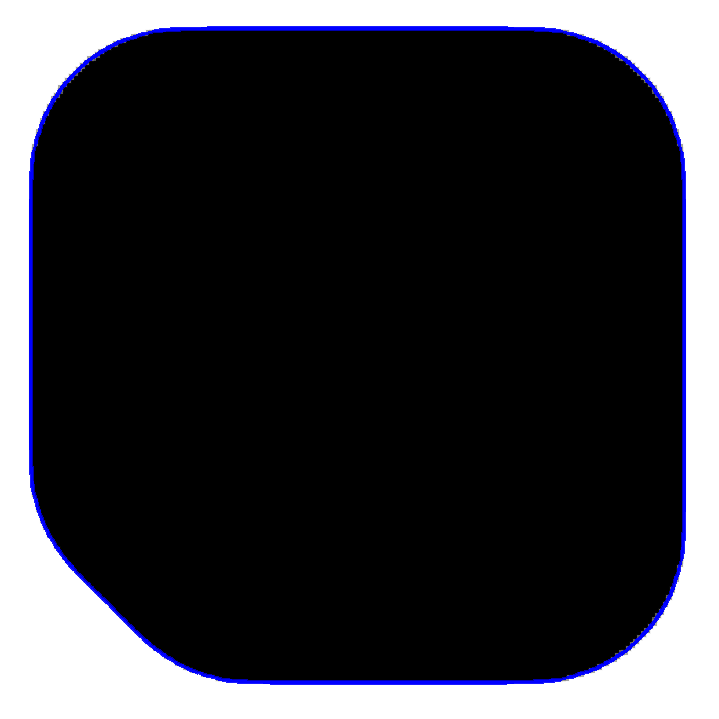
\includegraphics[width=.22\linewidth]{cheeger-weight/square-constant-bump4-cheeger-curve.png}
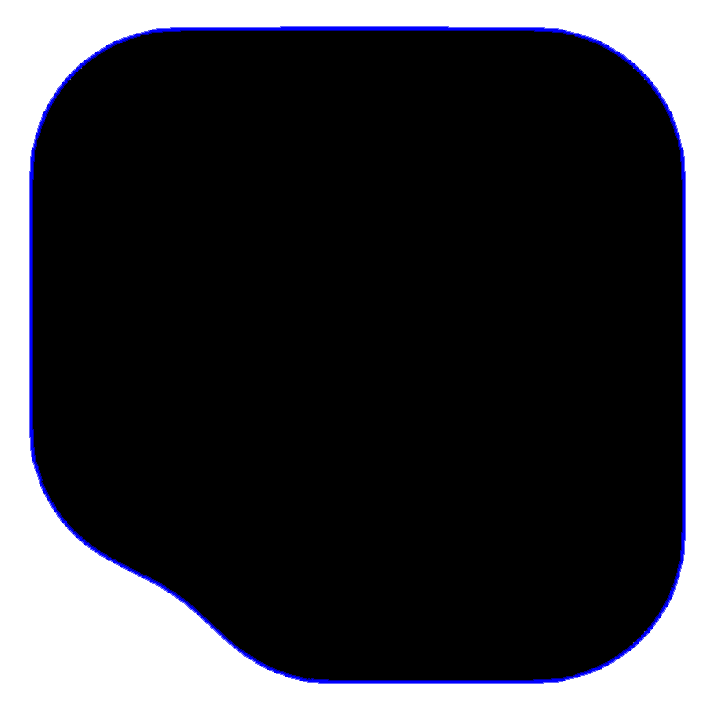
\includegraphics[width=.22\linewidth]{cheeger-weight/square-constant-bump3-cheeger-curve.png}

\includegraphics[width=.22\linewidth]{cheeger-weight/square-constant-bump2-cheeger-curve.png}
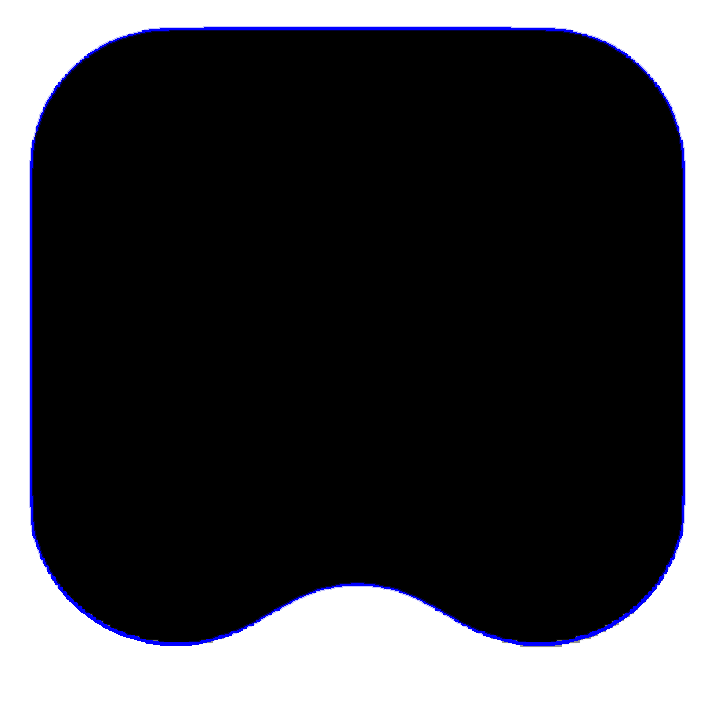
\includegraphics[width=.22\linewidth]{cheeger-weight/square-constant-bump1-cheeger-curve.png}
}{
Cheeger sets in a 2D square with $f=1$ and several non-constant weights $g$.
}{fig-cheeger-bump}



\myfigure{
\begin{tabular}{cccc}
\hspace{-3mm}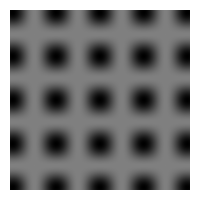
\includegraphics[width=.23\linewidth]{cheeger-weight/square-constant-periodic-tv.png}&
\hspace{-3mm}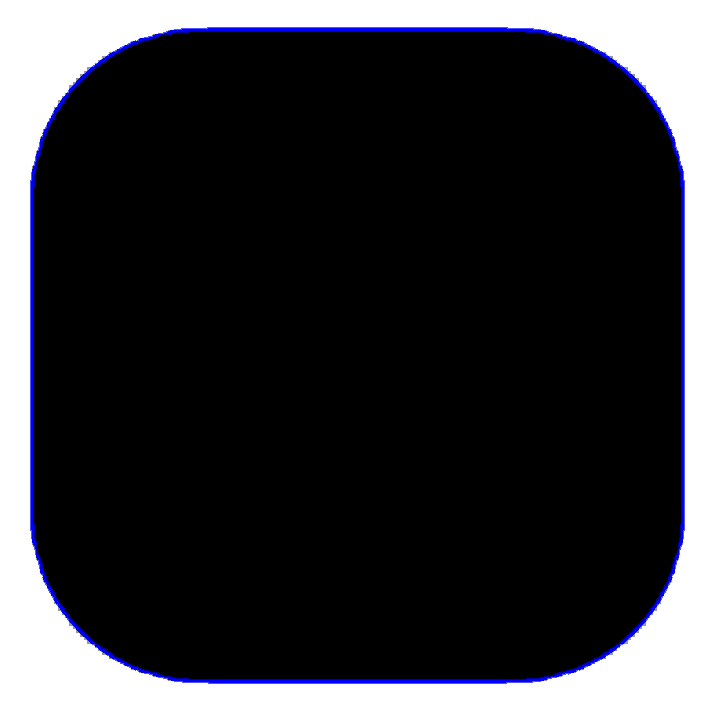
\includegraphics[width=.23\linewidth]{cheeger-2d/square-l2-cheeger-curve.png}&
\hspace{-3mm}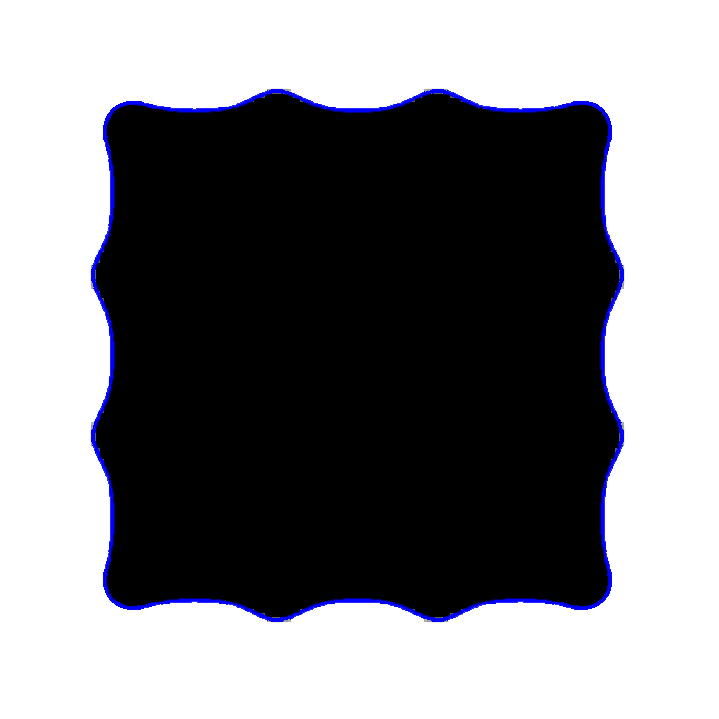
\includegraphics[width=.23\linewidth]{cheeger-weight/square-constant-periodic-cheeger-curve.png}&
\hspace{-3mm}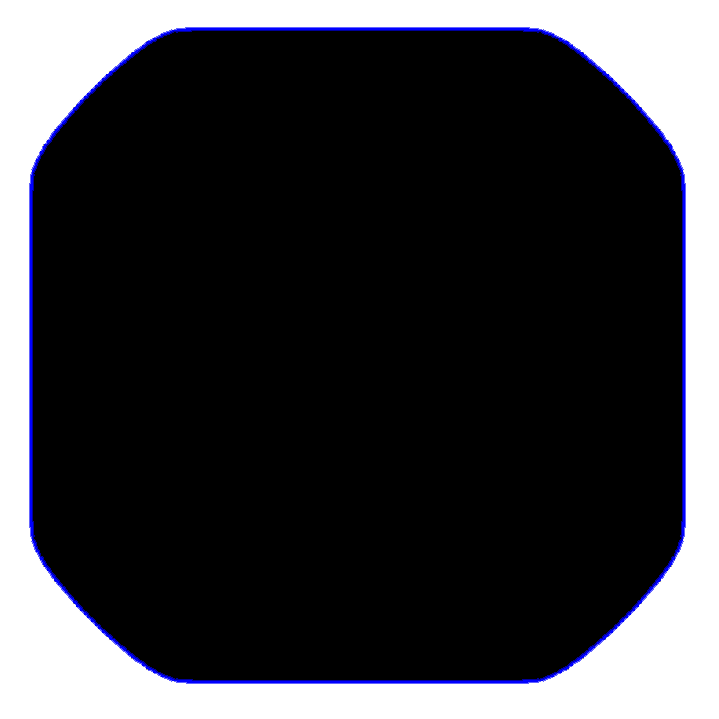
\includegraphics[width=.23\linewidth]{cheeger-weight/square-periodic-constant-cheeger-curve.png}\\
\hspace{-3mm}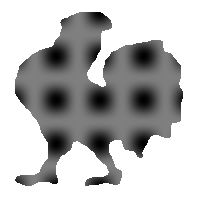
\includegraphics[width=.23\linewidth]{cheeger-weight/chicken-constant-periodic-tv.png}&
\hspace{-3mm}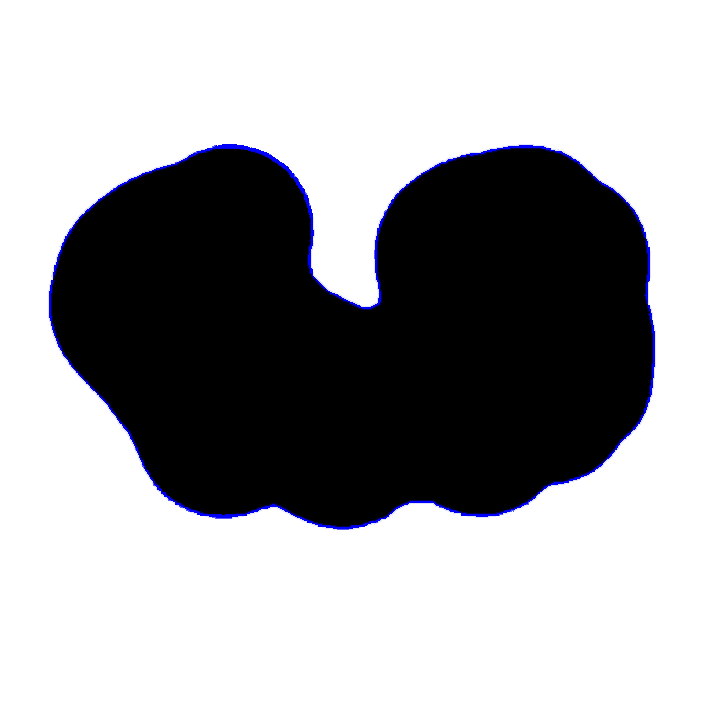
\includegraphics[width=.23\linewidth]{cheeger-2d/chicken-l2-cheeger-curve.png}&
\hspace{-3mm}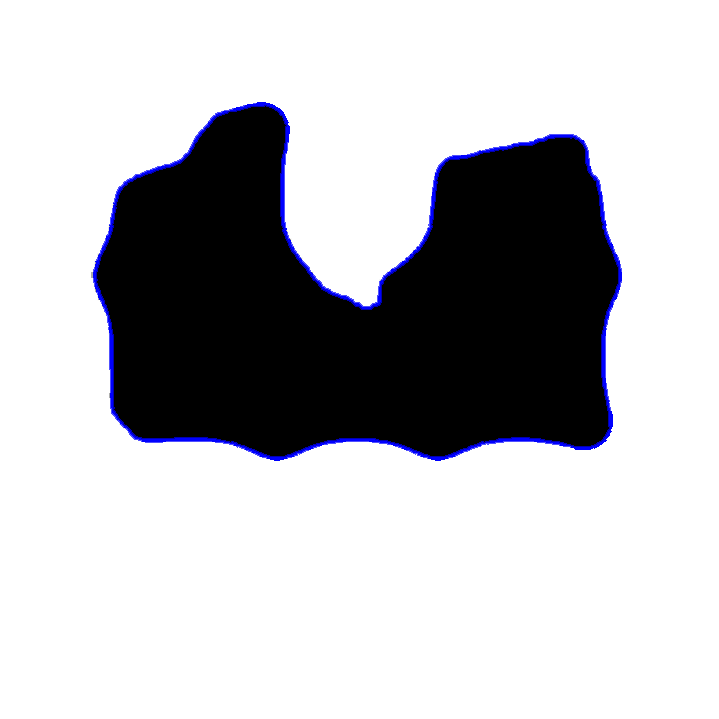
\includegraphics[width=.23\linewidth]{cheeger-weight/chicken-constant-periodic-cheeger-curve.png}&
\hspace{-3mm}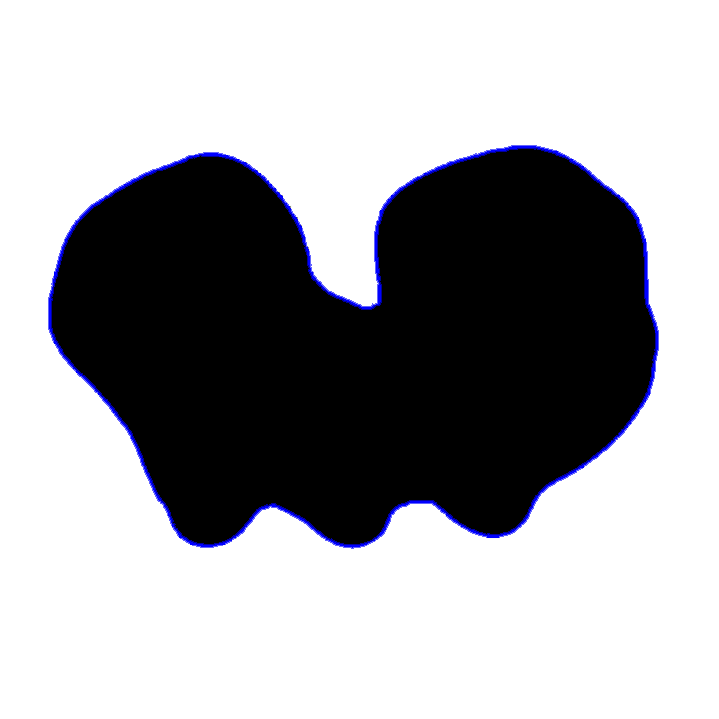
\includegraphics[width=.23\linewidth]{cheeger-weight/chicken-periodic-constant-cheeger-curve.png}\\
Weight $w$ & $f=g=1$ & $g=w, f=1$ & $g=1, f=w$
\end{tabular}
}{
Comparison of the Cheeger with constant weights and with varying weights $g$ or $f$.
}{fig-cheeger-weight}





\paragraph{Crystalline total variation.}

The Cheeger extraction algorithm presented in this paper can be extended to handle non isotropic total variation (see \cite{bccn}). Such a total variation is defined as
\begin{equation*}
	G_{\phi}(u) = \int_{\Omega} \phi( \nabla u) 
\end{equation*}
where $\phi : \mathbb{R}^2�\mapsto \mathbb{R}^+$ is a convex, continuous, and positively homogeneous function. In the numerical simulation we consider the L$^1$ and L$^\infty$ crystalline total variation $G_1$ and $G_\infty$ which corresponds to taking $\phi$ equal respectively to
\begin{equation*}
	\norm{(x_1,x_2)}_1 = |x_1|+|x_2|
	\quad\text{and}\quad
	\norm{(x_1,x_2)}_\infty = \max(|x_1|,|x_2|).
\end{equation*}
The discrete projection algorithm presented in section \ref{subsec-algorithm} can be used in order to compute the Cheeger for a crystalline norm. The only modification is that the sub-gradient $t^{(k)}$ computed following \eqref{eq-subgradient-tv} should be modified as follow
\begin{equation*}
	t^{(k)} = \frac{1}{\sqrt{f}} \div\left( g \phi^*(\nabla \tilde u^{(k)})  \right),
\end{equation*}
where the function $\phi^* : \mathbb{R}^2 \rightarrow \mathbb{R}^2$ is defined differently for the L$^1$ and L$^\infty$ total variations
\begin{align*}
	\phi^*_1(x_1,x_2) &= (\sign(x_1),\sign(x_2)) \\
	\phi^*_\infty( (x_1,x_2) ) &= 
		\left\{
		\begin{array}{l}
			(\sign(x_1),0) \text{ if } |x_1|>|x_2|,\\
			(0,\sign(x_2)) \text{ otherwise}.
		\end{array}
		\right. 
\end{align*}
Figure \ref{fig-cheeger-2d}, third and fourth rows, show examples of Cheeger sets for 2D shapes with constant weights $f=g=1$ and crystalline total variations.

\myfigure{
\begin{tabular}{cccc}
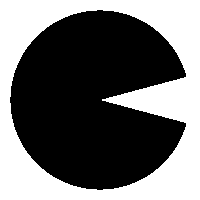
\includegraphics[width=.23\linewidth]{cheeger-2d/pacman-original.png}&
\hspace{-3mm}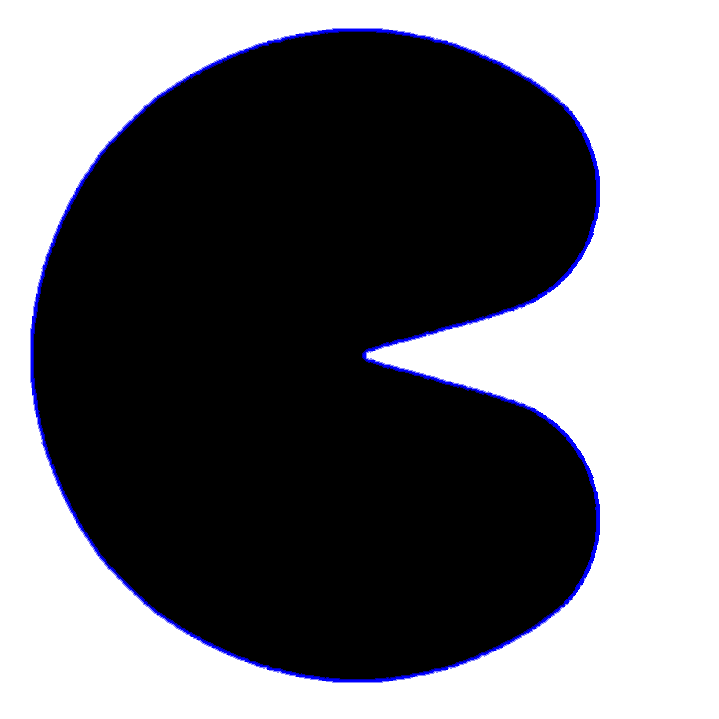
\includegraphics[width=.23\linewidth]{cheeger-2d/pacman-l2-cheeger-curve.png}&
\hspace{-3mm}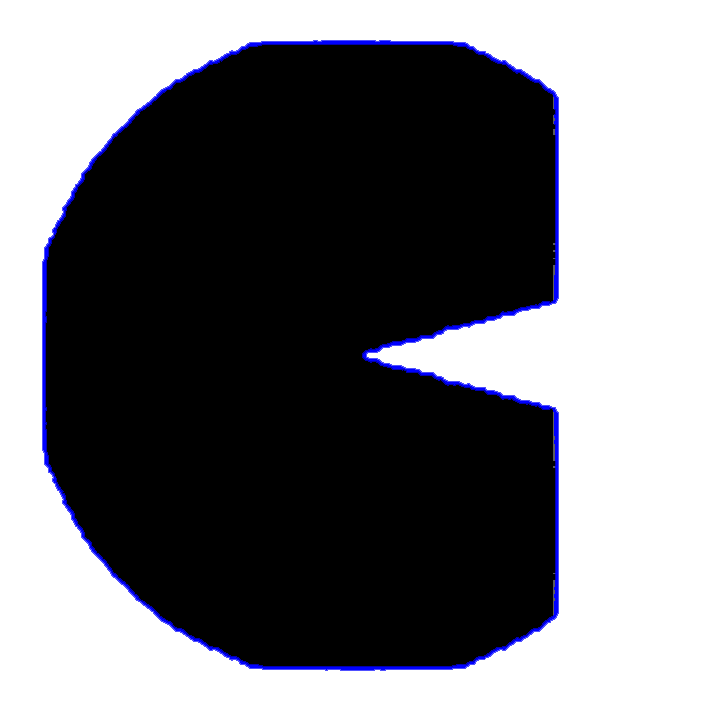
\includegraphics[width=.23\linewidth]{cheeger-2d/pacman-l1-cheeger-curve.png}&
\hspace{-3mm}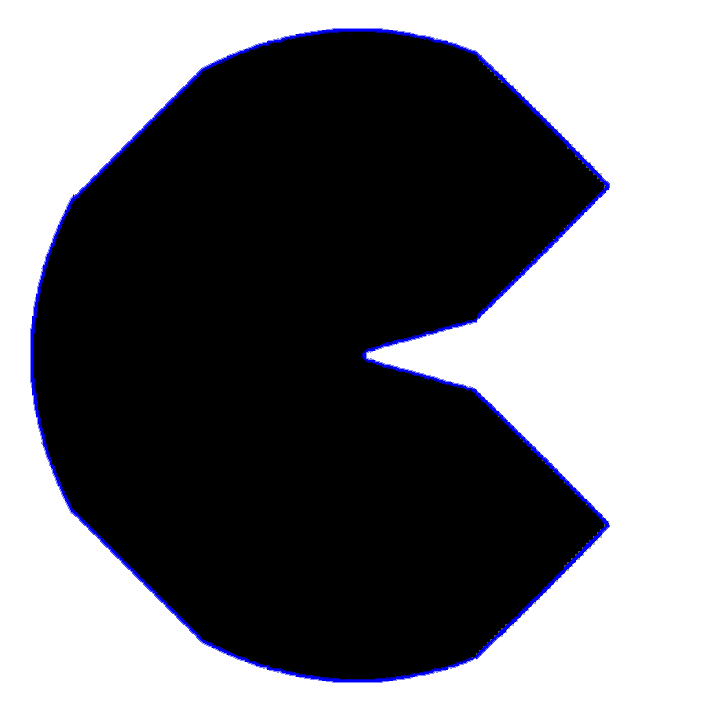
\includegraphics[width=.23\linewidth]{cheeger-2d/pacman-linf-cheeger-curve.png}\\[-2.5mm]
%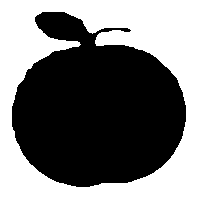
\includegraphics[width=.23\linewidth]{cheeger-2d/apple-original.png}&
%\hspace{-3mm}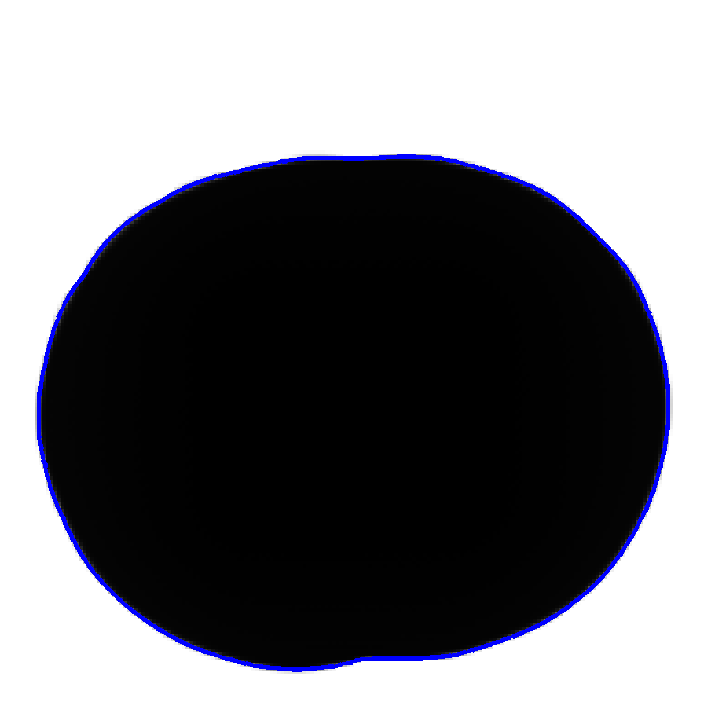
\includegraphics[width=.23\linewidth]{cheeger-2d/apple-l2-cheeger-curve.png}&
%\hspace{-3mm}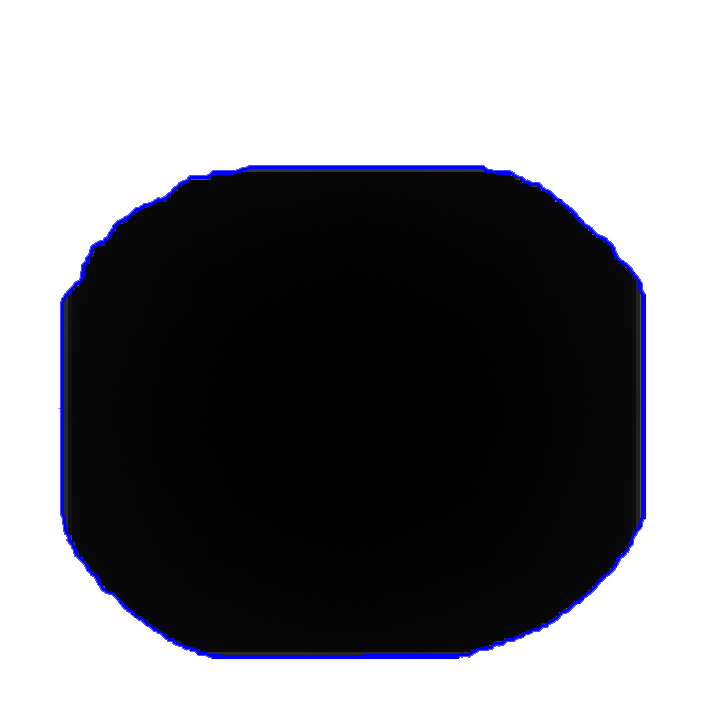
\includegraphics[width=.23\linewidth]{cheeger-2d/apple-l1-cheeger-curve.png}&
%\hspace{-3mm}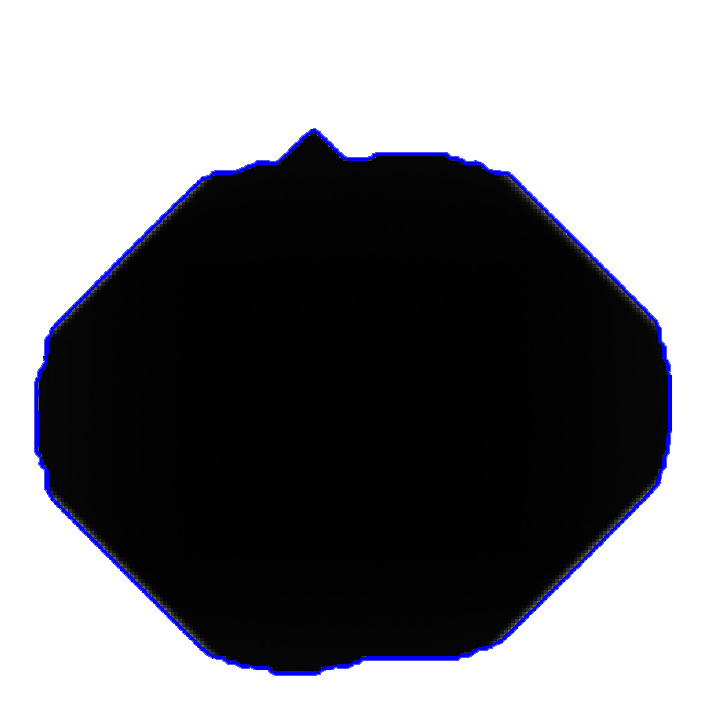
\includegraphics[width=.23\linewidth]{cheeger-2d/apple-linf-cheeger-curve.png}\\[-3mm]
%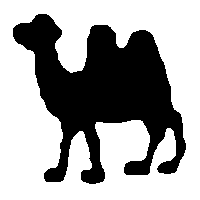
\includegraphics[width=.23\linewidth]{cheeger-2d/camel-original.png}&
%\hspace{-3mm}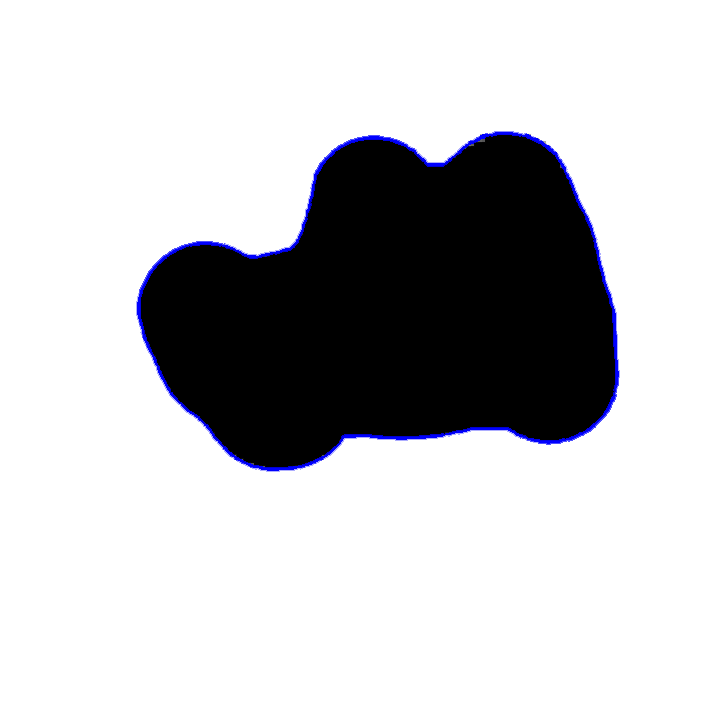
\includegraphics[width=.23\linewidth]{cheeger-2d/camel-l2-cheeger-curve.png}&
%\hspace{-3mm}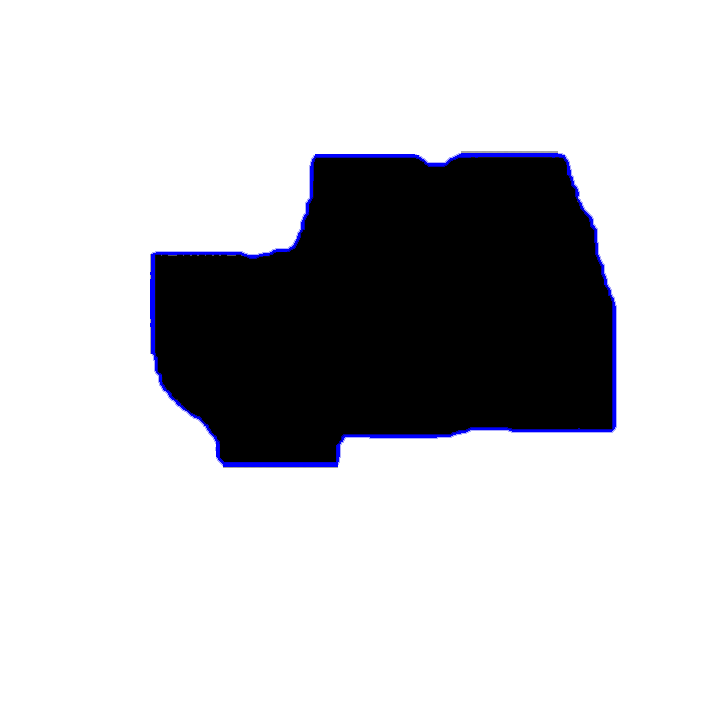
\includegraphics[width=.23\linewidth]{cheeger-2d/camel-l1-cheeger-curve.png}&
%\hspace{-3mm}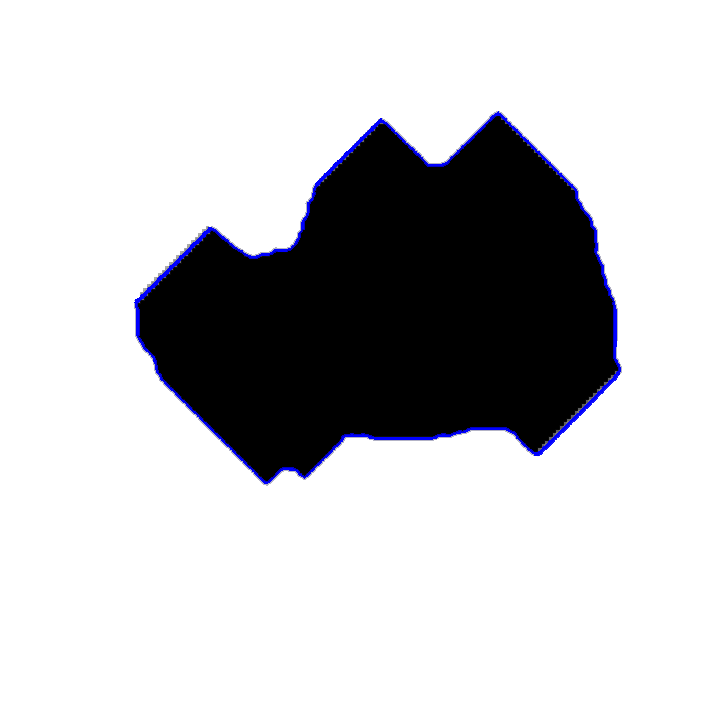
\includegraphics[width=.23\linewidth]{cheeger-2d/camel-linf-cheeger-curve.png}\\[-3mm]
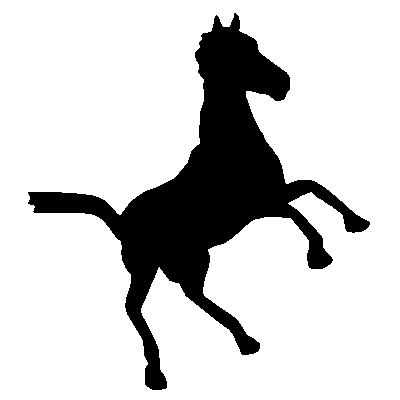
\includegraphics[width=.23\linewidth]{cheeger-2d/horse-original.png}&
\hspace{-3mm}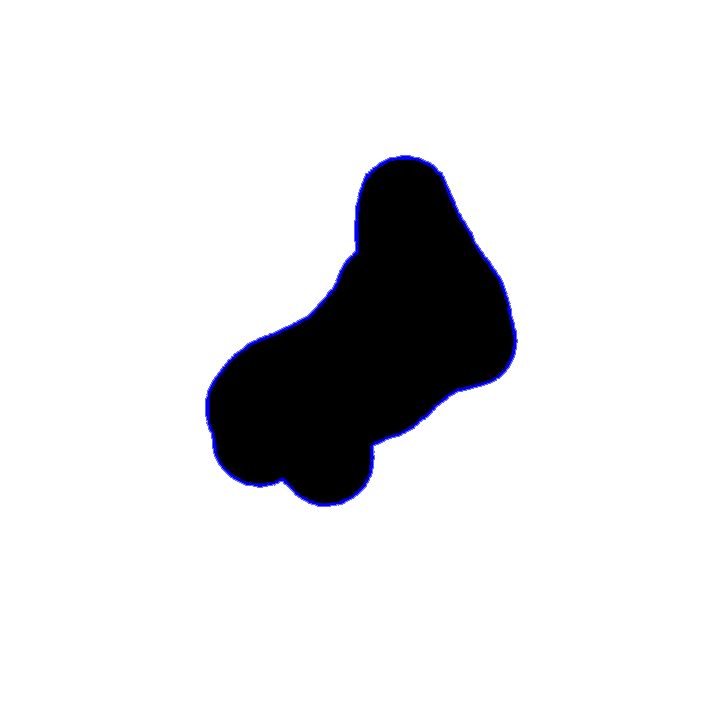
\includegraphics[width=.23\linewidth]{cheeger-2d/horse-l2-cheeger-curve.png}&
\hspace{-3mm}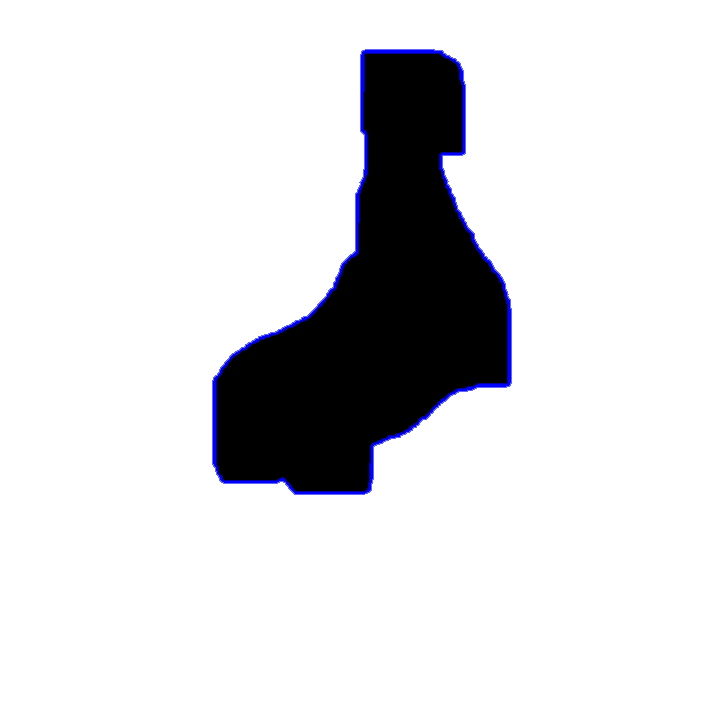
\includegraphics[width=.23\linewidth]{cheeger-2d/horse-l1-cheeger-curve.png}&
\hspace{-3mm}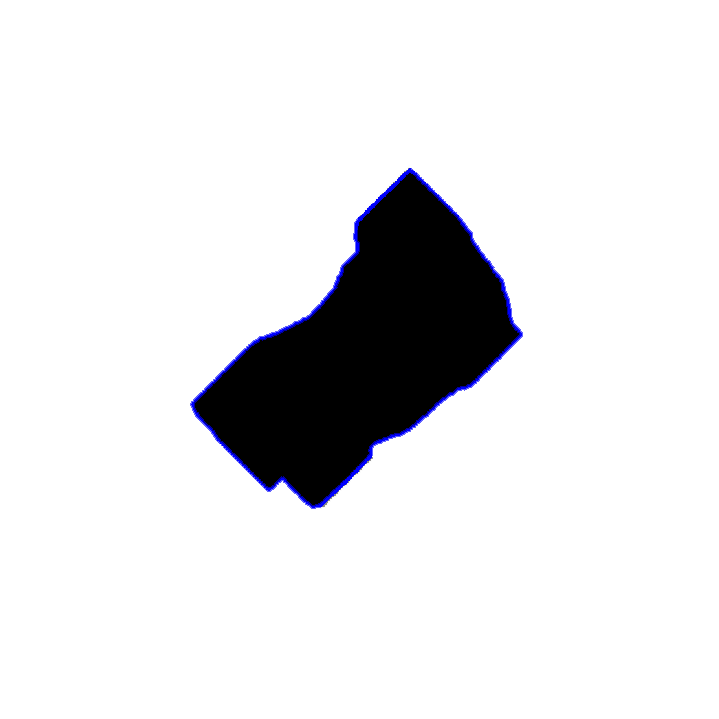
\includegraphics[width=.23\linewidth]{cheeger-2d/horse-linf-cheeger-curve.png}\\[-2.5mm]
%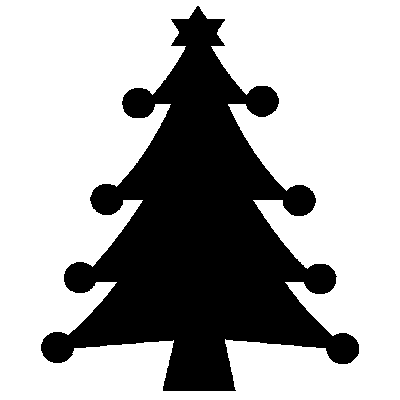
\includegraphics[width=.23\linewidth]{cheeger-2d/sapin-original.png}&
%\hspace{-3mm}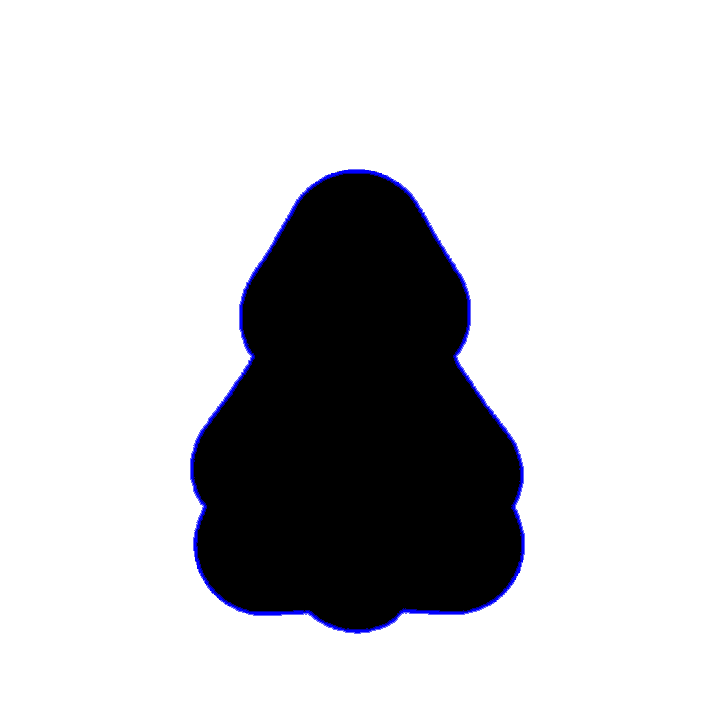
\includegraphics[width=.23\linewidth]{cheeger-2d/sapin-l2-cheeger-curve.png}&
%\hspace{-3mm}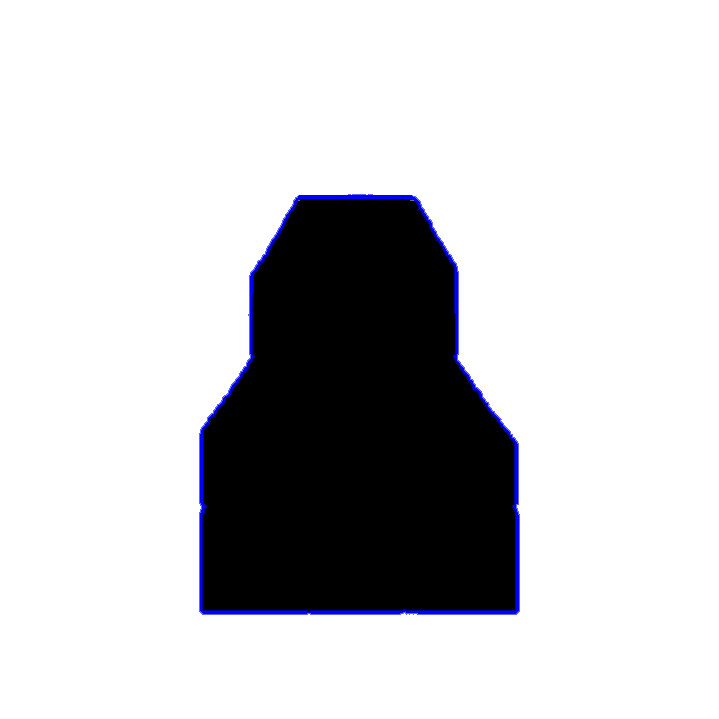
\includegraphics[width=.23\linewidth]{cheeger-2d/sapin-l1-cheeger-curve.png}&
%\hspace{-3mm}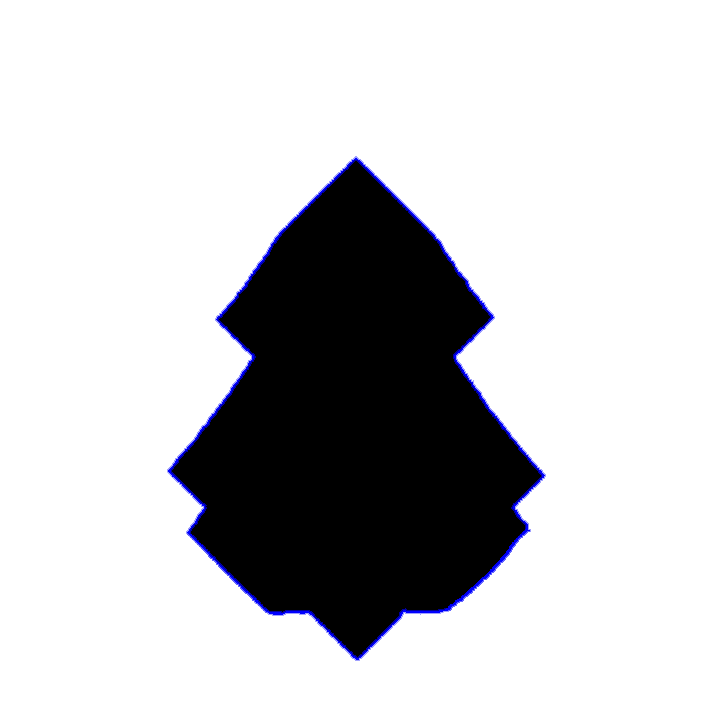
\includegraphics[width=.23\linewidth]{cheeger-2d/sapin-linf-cheeger-curve.png}\\
Shape & L$^2$ cheeger & L$^1$ cheeger & L$^\infty$ cheeger
\end{tabular}
}{
Cheeger sets in 2D with constant weights $f=g=1$ and for both euclidean (second row) and crystalline (third and fourth row) total variation.
}{fig-cheeger-2d}




%%%%%%%%%%%%%%%%%%%%%%%%%%%%%%%%%%%%%%%%%%%%%%%%%%%%%%%%%%%%%%
%%%%%%%%%%%%%%%%%%%%%%%%%%%%%%%%%%%%%%%%%%%%%%%%%%%%%%%%%%%%%%
%%%%%%%%%%%%%%%%%%%%%%%%%%%%%%%%%%%%%%%%%%%%%%%%%%%%%%%%%%%%%%
\begin{thebibliography}{999}



\bibitem{ac} F. Alter, V. Caselles, \textit{Uniqueness of the Cheeger set of a convex body}, preprint available at {\tt http://cvgmt.sns.it} (2007). 

\bibitem{acc} F.Alter, V. Caselles and A. Chambolle, \textit{Evolution of characteristic functions of convex sets in the plane by the minimizing total variation flow},  Interfaces Free Bound., \textbf{7},  no. 1, pp.~29--53 (2005).

\bibitem{afp}L.~Ambrosio, N.~Fusco, D.~Pallara: {\it Functions of Bounded
Variation and Free Discontinuity Problems.} Oxford Mathematical Monographs,
Oxford University Press, New York (2000).


\bibitem{appleton} B. Appleton and H. Talbot, \textit{Globally Minimal Surfaces by Continuous Maximal Flows}, IEEE Trans. Pattern Analysis and Machine Intelligence, \textbf{28}, no. 1, pp.~106-118 (2006).

\bibitem{bccn} G. Bellettini, V. Caselles, A. Chambolle, and M. Novaga, \textit{Crystalline mean curvature flow of convex sets},  Arch. Ration. Mech. Anal., \textbf{179},  no. 1, pp.~109--152 (2006). 


\bibitem{bcc} G. Buttazzo, G. Carlier and  M. Comte, \textit{On the selection of maximal Cheeger sets},   Differential and Integral Equations, \textbf{20},  no 9, pp.~991-1004 (2007).

\bibitem{cc} G. Carlier and M. Comte, \textit{On a weighted total variation minimization problem}, J. Funct. Anal., \textbf{250}, pp.~214-226 (2007).


\bibitem{ccn}V.~Caselles, A.~Chambolle and M.~Novaga, \textit{Uniqueness of the Cheeger set of a convex body},  Pacific J. Math., \textbf{232},  no. 1, pp.~77--90 (2007) .


\bibitem{chambolle} A. Chambolle, \textit{An algorithm for total variation minimization and applications},  Special issue on mathematics and image analysis.  J. Math. Imaging Vision,  \textbf{20} ,  no. 1-2, pp.~89--97 (2004).

\bibitem{cl} A. Chambolle, P.-L. Lions, \textit{Image recovery via total variation minimization}, Numer. Math., \textbf{76}, pp.~167-188 (1997).

\bibitem{cp} P.-L. Combettes and J.-C. Pesquet, \textit{Image Restoration Subject to a Total Variation Constraint},  IEEE Transactions on Image Processing, \textbf{13}, no. 9, pp.~1213-1222 (2004).

\bibitem{comb} P.-L. Combettes, \textit{A block-iterative surrogate constraint splitting method for quadratic signal recovery}, IEEE Transactions on Signal Processing, \textbf{51}, no. 7, pp.~1771-1782 (2003).

\bibitem{cris}N. Cristescu,  {\it A model of stability of slopes} in Slope Stability 2000, , Proceedings of Sessions of Geo-Denver 2000, D. V. Griffiths, G. A. Fenton, T. R. Martin, (eds). Geotechnical special publication,  {\bf 101}, pp.~86--98 (2000).

\bibitem{dem1} F. Demengel, {\it Th\'eor\`emes d'existence pour des \'equations avec l'op\'erateur "1-Laplacien", premi\`ere valeur propre de $-\Delta\sb 1$}, C.R Math. Acad. Sci. Paris, \textbf{334},  12, pp.~1071--1076 (2002).

\bibitem{dem2} F. Demengel, {\it Some existence's results for noncoercive "1-Laplacian" operator}, Asymptotic Analysis, \textbf{43},  pp.~287--322 (2005).


\bibitem {ektem}I. Ekeland, R. Temam, \textit{Convex Analysis and Variational
Problems}, Classics in Mathematics, Society for Industrial and Applied
Mathematics, Philadelphia, (1999).


\bibitem{eg} L.C. Evans and R. Gariepy, \textit{ Measure Theory and Fine Properties of Functions}, CRC Press (1992).


\bibitem{duli} G. Duvaut and J.-L. Lions, \textit{ Les in\'equations en m\'ecanique et en physique}, Dunod, Paris (1972).

\bibitem{hilr} R. Hassani, I.R. Ionescu and T. Lachand-Robert, \textit{Shape optimization and Supremal Minimization Approaches in Landslides Modeling}, Applied Mathematics and Optimization, \textbf{52}, 3, pp.~349--364  (2005).


\bibitem{hilrr}P. Hild, I.R. Ionescu, T. Lachand-Robert and I. Rosca \textit{ The blocking of an inhomogeneous Bingham fluid. Applications to landslides},  Mathematical Modelling and Numerical Analysis (M2AN), \textbf{36}, 6, pp.~1013-1026 (2002).

\bibitem{lri} I. R. Ionescu and  T. Lachand-Robert,
\textit{Generalized Cheeger sets related to landslides}, Calc. Var. and PDE's \textbf{23}, pp.~227--249 (2005).

\bibitem{nozawa}  R. Nozawa, \textit{Max-flow min-cut theorem in an anisotropic network}, Osaka J. Math., \textbf{27},  pp.~805-842 (1990). 

\bibitem{rof} L.I. Rudin, S. Osher, E. Fatemi, \textit{Nonlinear total variation based noise removal algorithms}, Physica D, \textbf{60}, pp.~259-268 (1992). 

\bibitem{strang1} G. Strang, \textit{Maximal flow through a domain}, Math. Programming, \textbf{26},  pp.~123-143, (1983).

\bibitem{strang2} G. Strang, \textit{Maximum flows and minimum cuts in the plane}, to appear in Journal of Global Optimization (2007). 
 
 
\end{thebibliography}

\end{document}
